\chapter{Descripción}

\section{Análisis de los resultados de la encuesta}

Con el objetivo de relevar la percepción de los usuarios respecto de la
administración y optimización de recursos en entornos de computación en
la nube, se realizó una encuesta mediante Google Forms. Se obtuvieron un
total de 48 respuestas. El cuestionario permitió recopilar información
tanto de usuarios con experiencia práctica en la administración de
infraestructura cloud como de personas sin experiencia directa,
diferenciando posteriormente ambos grupos para evitar que la falta de
experiencia condicionara el análisis de las preguntas de carácter
técnico. Los resultados completos y las respuestas individuales se
presentan en el Anexo correspondiente.

En primer lugar, se analizó la existencia de dificultades relacionadas
con la utilización eficiente de los recursos cloud. De los 48
participantes, 15 manifestaron contar con experiencia práctica en la
administración de infraestructura en la nube. Dentro de este grupo, 10
participantes indicaron haber experimentado gastos inesperados o
sobrecostos asociados al uso de servicios cloud, mientras que los 5
restantes indicaron no haber atravesado esta situación. En consecuencia,
aproximadamente el 66,7 \% de los participantes con experiencia práctica
manifestó haber experimentado algún grado de sobrecosto. Este resultado
permite observar que los costos derivados de una utilización ineficiente
de los recursos constituyen una problemática presente entre los usuarios
con experiencia en este tipo de infraestructura.

Se consultó a los participantes con experiencia sobre la dificultad para
identificar recursos ineficientes dentro de una infraestructura cloud,
utilizando una escala de 1 a 5. Las respuestas se concentraron
principalmente en los valores intermedios y altos, obteniéndose un
promedio de 3,56 sobre 5. Esto permite caracterizar la identificación de
recursos ineficientes como una tarea de dificultad moderada a elevada.

En relación con las métricas utilizadas para evaluar el estado de los
recursos, los costos fueron el indicador mencionado con mayor frecuencia
entre los participantes con experiencia, seguido por el uso de CPU y el
almacenamiento. La memoria RAM también presentó una frecuencia elevada,
mientras que variables como la disponibilidad, el tráfico de red y el
uso de contenedores tuvieron una presencia menor. Estos resultados
respaldan la selección inicial de métricas consideradas por la solución
propuesta, particularmente aquellas relacionadas con el consumo de CPU,
memoria y almacenamiento, complementadas por información económica
asociada a los recursos.

Por otra parte, se relevó qué herramientas utilizan actualmente los
participantes con experiencia práctica para monitorear, administrar y
optimizar sus infraestructuras cloud. Entre las soluciones mencionadas
se encontraron herramientas ampliamente reconocidas en el mercado, como
Grafana, Amazon CloudWatch, Datadog, Prometheus, Kubernetes Dashboard,
New Relic y Terraform. Resulta particularmente relevante que varios de
los participantes con experiencia práctica indicaron utilizar
herramientas que constituyen alternativas o competidores directos
respecto de distintas funcionalidades contempladas en la solución
propuesta. Por ejemplo, Datadog y New Relic ofrecen capacidades de
monitoreo y observabilidad, mientras que Amazon CloudWatch proporciona
servicios de monitoreo sobre infraestructura de AWS. La presencia de
estas herramientas entre las respuestas permite considerar que una parte
de la muestra posee conocimiento y experiencia real con soluciones
existentes en el mercado, por lo que sus respuestas aportan una
perspectiva relevante para evaluar las necesidades y limitaciones de las
alternativas actuales. A su vez, la diversidad de herramientas
utilizadas evidencia que los usuarios recurren a diferentes soluciones
para cubrir necesidades específicas de monitoreo, visualización,
administración e infraestructura como código. Esta posible fragmentación
resulta relevante para la propuesta desarrollada, que busca integrar en
una misma plataforma el análisis de utilización de recursos, la
detección de ineficiencias, la generación de recomendaciones de
optimización y la automatización mediante infraestructura como código.

Respecto de las principales limitaciones percibidas en las herramientas
utilizadas actualmente, la complejidad fue el aspecto mencionado con
mayor frecuencia, seguida por los costos elevados y la poca capacidad de
visualización. También se identificaron dificultades relacionadas con la
integración entre herramientas y con la utilidad de algunas de las
recomendaciones proporcionadas por las soluciones existentes. Estos
resultados permiten observar que la problemática no se limita
exclusivamente a la disponibilidad de métricas, sino que también
comprende la capacidad de interpretar dicha información y transformarla
en acciones concretas de optimización. En este sentido, una solución que
únicamente presente métricas o detecte anomalías podría resultar
insuficiente si no proporciona información que facilite la toma de
decisiones.

La encuesta también permitió analizar el interés de los participantes
respecto de las funcionalidades que podría ofrecer una plataforma
orientada a la optimización de recursos cloud. Las funcionalidades
seleccionadas con mayor frecuencia fueron el monitoreo del uso de
recursos y la generación de recomendaciones para optimizar costos, ambas
mencionadas por 27 participantes. A continuación, se ubicó la detección
automática de desperdicio de recursos, seleccionada por 20
participantes. También se identificó interés en funcionalidades
relacionadas con la generación de reportes y visualizaciones, la
automatización de despliegues y las alertas. Estos resultados presentan
una correspondencia directa con los objetivos de la solución propuesta,
dado que las principales funcionalidades demandadas pueden organizarse
en un flujo compuesto por la observación del comportamiento de los
recursos, la detección de situaciones ineficientes y la generación de
recomendaciones orientadas a su optimización.

Un aspecto particularmente relevante fue la valoración general de una
plataforma destinada a administrar recursos cloud de manera más
eficiente. Sobre el total de 48 participantes, 37 calificaron su
utilidad con un valor de 4 o 5 sobre 5, lo que representa
aproximadamente el 77,1 \% de la muestra, mientras que la valoración
promedio obtenida fue de 4 sobre 5. Entre los 15 participantes que
declararon contar con experiencia práctica en la administración de
infraestructura cloud, 12 calificaron la utilidad de la plataforma con 4
o 5, lo que representa el 80 \% de este grupo. Por otro lado, las cinco
valoraciones más bajas, correspondientes a valores de 1 o 2, provinieron
tanto de participantes con experiencia como de participantes sin
experiencia, por lo que no se observa que el rechazo hacia la propuesta
esté concentrado exclusivamente en alguno de estos grupos. En conjunto,
estos resultados evidencian un nivel elevado de interés potencial en una
solución orientada a facilitar la administración eficiente de recursos
cloud.

Sin embargo, la aceptación de las recomendaciones automatizadas presentó
un comportamiento más moderado. La confianza promedio declarada por los
participantes fue de 3,44 sobre 5, mientras que el 50 \% de la muestra
otorgó una valoración de 4 o 5. Al analizar específicamente a los
participantes con experiencia práctica en infraestructura cloud, este
porcentaje se incrementó al 66,7 \%. Esto permite identificar una
diferencia entre el interés por utilizar una herramienta de optimización
y la disposición a delegar decisiones de infraestructura en un sistema
automatizado. En consecuencia, los resultados sugieren que la
automatización constituye una funcionalidad valorada, pero debe estar
acompañada por mecanismos que permitan al usuario comprender, revisar y
controlar las acciones recomendadas.

La seguridad se identificó como el principal factor que condiciona la
confianza en las recomendaciones automatizadas, siendo mencionada por 24
participantes. Otros factores señalados fueron el riesgo de errores, la
experiencia previa, los costos y la falta de transparencia. Este
resultado tiene implicancias directas sobre el diseño de la solución
propuesta. En lugar de plantear una modificación automática e
irreversible de la infraestructura, resulta conveniente adoptar un
enfoque basado en recomendaciones explicables y controladas por el
usuario. Bajo este enfoque, el sistema puede detectar una situación
potencialmente ineficiente, explicar los datos que justifican la
recomendación, proponer una acción de optimización y, posteriormente,
permitir al usuario decidir si desea aplicarla.

Esta consideración resulta especialmente relevante para la integración
con Terraform planteada en el proyecto. En lugar de modificar
directamente los recursos productivos, la plataforma puede utilizar los
resultados del análisis para generar una propuesta de infraestructura
como código optimizada. De esta manera, el usuario conserva el control
sobre el cambio y puede revisar el código generado antes de aplicarlo.
Este mecanismo permite combinar automatización con supervisión humana,
reduciendo el riesgo asociado a modificaciones automáticas sobre
infraestructura crítica.

En conjunto, los resultados obtenidos permiten identificar tres aspectos
principales. En primer lugar, existe evidencia de que los usuarios con
experiencia en infraestructura cloud enfrentan problemas relacionados
con sobrecostos y con la identificación de recursos ineficientes. En
segundo lugar, las funcionalidades consideradas más relevantes por los
participantes monitoreo, optimización de costos y detección automática
de desperdicio presentan una correspondencia directa con los objetivos
de la solución propuesta. Finalmente, aunque existe una valoración
positiva hacia una plataforma de este tipo, la confianza en las
recomendaciones automatizadas se encuentra condicionada principalmente
por cuestiones de seguridad y transparencia.

Por lo tanto, los resultados de la encuesta proporcionan evidencia
favorable para continuar con el desarrollo de una plataforma orientada a
la detección de ineficiencias en infraestructuras cloud y a la
generación de recomendaciones de optimización. Al mismo tiempo, permiten
establecer criterios de diseño que trascienden la detección de
anomalías: las recomendaciones deben ser comprensibles, justificables y
revisables por el usuario, y las acciones de modificación de
infraestructura deberían mantener un mecanismo de supervisión antes de
su aplicación. De esta manera, la encuesta no solo contribuye a validar
la problemática abordada, sino que también aporta evidencia para definir
las características funcionales y de seguridad de la solución
desarrollada.

\section{Análisis de entrevistas}

Se realizó un análisis exhaustivo de tres entrevistas semiestructuradas realizadas a profesionales especializados en la administración de infraestructura cloud, específicamente dentro del ecosistema de Huawei Cloud. Estas entrevistas fueron diseñadas con el objetivo de comprender en profundidad los desafíos actuales que enfrentan los administradores de infraestructura cloud, las metodologías empleadas para la gestión de recursos, los problemas relacionados con costos y eficiencia, así como las expectativas y requisitos que dichos profesionales tienen respecto a herramientas de optimización basadas en inteligencia artificial. El análisis aquí presentado busca identificar patrones comunes, extraer insights significativos y proporcionar una base sólida para el desarrollo de soluciones tecnológicas que aborden las necesidades detectadas.

Las entrevistas fueron conducidas con tres profesionales que ocupan roles diferenciados dentro del ecosistema de Huawei Cloud, lo cual proporciona una perspectiva multidimensional del fenómeno estudiado. Los participantes fueron seleccionados considerando su experiencia directa en administración de infraestructura cloud, su involucramiento en proyectos de optimización de recursos y su conocimiento especializado en herramientas de monitoreo y gestión de costos.

El instrumento de recolección de datos estuvo compuesto por un cuestionario estructurado que abordaba diez dimensiones temáticas: contexto actual de administración, planificación de recursos, monitoreo y operación, gestión de costos y eficiencia, detección de recursos innecesarios, herramientas utilizadas, confianza en recomendaciones automáticas, funcionalidades prioritarias, validación de propuestas y comentarios adicionales. Esta estructura permitió mantener consistencia en la recolección de datos mientras se preservaba la flexibilidad necesaria para explorar temas emergentes durante las conversaciones.

El primer participante, Donnie Sacristan, se desempeña como IT Manager en Hiberus, empresa que opera como cliente de Huawei Cloud. Su rol implica la responsabilidad directa sobre la administración de infraestructura cloud en un entorno multicloud, caracterizado por la presencia de múltiples proveedores de servicios en la nube. Esta configuración arquitectónica representa un escenario de complejidad elevada, donde la gestión unificada de recursos distribuidos entre diferentes plataformas constituye un desafío operativo significativo. Donnie ha desarrollado soluciones personalizadas para consolidar información proveniente de distintas cuentas cloud, lo cual evidencia su capacidad técnica y su comprensión profunda de las limitaciones de las herramientas nativas para entornos multicloud.

El segundo participante, Agustín Chiarenza, trabaja para Huawei Cloud en el contexto del cliente OCA, una organización de gran envergadura con infraestructura cloud extensa. Su participación en el desarrollo de un agente de inteligencia artificial orientado a la automatización de procesos de FinOps proporciona una perspectiva única desde el lado de la creación de soluciones tecnológicas. Agustín posee conocimiento detallado sobre la arquitectura del agente desarrollado, sus capacidades técnicas, las fuentes de datos que integra y los resultados obtenidos en su implementación. Su testimonio resulta particularmente valioso para comprender las decisiones de diseño, las limitaciones encontradas y el potencial de escalabilidad de este tipo de soluciones.

El tercer participante, Nicolás Irigoyen, ocupa el rol de arquitecto de soluciones cloud especializado en inteligencia artificial dentro de Huawei Cloud. Su perspectiva difiere de los participantes anteriores en tanto que su trabajo se centra en el diseño y prueba de soluciones más que en la administración operativa de infraestructura productiva. Nicolás administra sus propios recursos de manera individual, lo cual proporciona una visión desde el rol de usuario individual de servicios cloud. Su especialización en inteligencia artificial le otorga una comprensión técnica avanzada sobre las capacidades y limitaciones de los sistemas automatizados, enriqueciendo el análisis con consideraciones sobre la viabilidad técnica de las soluciones propuestas.

\subsection{Entrevista con Donnie Sacristan - IT Manager en Hiberus}

La entrevista con Donnie Sacristan revela una realidad operativa caracterizada por la complejidad inherente a los entornos multicloud. Como IT Manager, su responsabilidad abarca la administración de infraestructura distribuida entre diferentes proveedores de servicios cloud, lo cual implica la necesidad de mantener visibilidad y control sobre recursos que residen en plataformas heterogéneas con interfaces, métricas y herramientas de gestión diferenciadas. Esta fragmentación del panorama de recursos genera una dispersión de información que dificulta la obtención de una visión consolidada del estado operacional y financiero de la infraestructura.

Ante esta problemática, Donnie desarrolló un aplicativo personalizado que permite consolidar la información proveniente de las distintas cuentas cloud en un punto centralizado de acceso. Esta solución artesanal evidencia una brecha significativa en las herramientas disponibles comercialmente, las cuales frecuentemente se especializan en un único proveedor, dejando a los administradores de entornos multicloud sin opciones integradas que satisfagan sus necesidades de gestión unificada. La iniciativa de desarrollar una solución propia representa una respuesta común ante la insuficiencia de herramientas de mercado, aunque implica costos de desarrollo y mantenimiento que podrían evitarse con soluciones comerciales adecuadas.

En relación con la planificación de recursos, Donnie describe un proceso colaborativo donde solicita a los equipos de desarrollo y arquitectura información sobre el alcance proyectado de los proyectos y los requerimientos técnicos de las aplicaciones. La referencia al uso extensivo de contenedores Docker indica una modernización de la plataforma de despliegue, donde los Dockerfiles proporcionan especificaciones técnicas que facilitan la estimación de recursos necesarios. Sin embargo, cuando esta información no está disponible o es insuficiente, se adopta una estrategia incremental que aprovecha la elasticidad característica de los entornos cloud, iniciando con configuraciones conservadoras y escalando progresivamente según las demandas observadas.

El monitoreo de recursos en un entorno multicloud presenta desafíos particulares que Donnie aborda mediante la implementación de Prometheus, una herramienta de monitoreo de código abierto que permite consolidar métricas de diferentes fuentes. Esta elección tecnológica refleja una tendencia hacia la adopción de soluciones agnósticas respecto al proveedor, que pueden integrar información de múltiples plataformas cloud sin depender de las herramientas nativas de cada proveedor. La consolidación de métricas en un dashboard unificado permite la configuración de alertas y la visualización del estado operacional sin necesidad de navegar entre múltiples interfaces, mejorando significativamente la eficiencia operativa.

Respecto a la gestión de costos, Donnie confirma haber experimentado situaciones de sobrecostos, un problema endémico en entornos cloud donde la facilidad de provisionamiento puede conducir a una proliferación no controlada de recursos. La solución implementada en este ámbito involucra un agente proporcionado por Huawei Cloud que consolida información de costos y realiza análisis mediante inteligencia artificial para identificar oportunidades de optimización. Este agente detecta recursos sobredimensionados, identifica equipos que podrían ser descontinuados por falta de utilización y proporciona recomendaciones de ajuste. La incorporación de inteligencia artificial en este proceso representa una automatización significativa de tareas que tradicionalmente requerían análisis manual extensivo.

La detección de recursos ociosos, innecesarios o sobredimensionados se realiza mediante la combinación de herramientas nativas de cada proveedor y la consolidación en Prometheus y Grafana. Esta arquitectura de monitoreo permite mantener visibilidad sobre el estado de todos los recursos sin necesidad de acceder individualmente a cada consola de administración. Donnie destaca la utilidad del agente de Huawei Cloud para identificar recursos que permanecen apagados durante períodos prolongados, información que resulta valiosa para decisiones de descontinuación o redimensionamiento. La confianza en las recomendaciones proporcionadas por el agente se fundamenta en la visualización de datos históricos que respaldan cada sugerencia, aspecto crítico para la aceptación de recomendaciones automatizadas.

Finalmente, Donnie plantea una necesidad no cubierta relacionada con la gestión de permisos y templates de infraestructura. La heterogeneidad de plataformas cloud implica que cada proveedor mantiene sus propios sistemas de templates y gestión de identidades, generando fragmentación que dificulta la administración unificada. La propuesta de una plataforma centralizada para gestionar permisos, usuarios y templates que se traduzca automáticamente a las especificaciones de cada nube representa una extensión natural del concepto de consolidación aplicado al monitoreo y costos, extendiéndolo al ámbito de la gobernanza y automatización de despliegues.

\subsection{Entrevista con Agustín Chiarenza - Desarrollador de Agente IA para OCA}

La entrevista con Agustín Chiarenza proporciona una perspectiva técnica detallada sobre el desarrollo e implementación de un agente de inteligencia artificial diseñado específicamente para automatizar procesos de FinOps en OCA, un cliente de gran envergadura de Huawei Cloud. El contexto que motiva el desarrollo de esta solución es la escala significativa de la infraestructura de OCA, donde la gestión manual de costos y optimización de recursos se vuelve impracticable debido al volumen y complejidad de los recursos involucrados. La decisión de desarrollar un agente basado en inteligencia artificial representa una apuesta tecnológica orientada a automatizar y facilitar procesos que de otra manera requerirían esfuerzos manuales extensivos.

La arquitectura del agente se fundamenta en la integración de herramientas nativas de Huawei Cloud, específicamente CloudEye y Cost Center. CloudEye es un servicio de monitoreo que se instala en todas las máquinas virtuales, proporcionando métricas detalladas sobre el consumo de recursos como CPU, memoria y tráfico de red. Cost Center, por su parte, proporciona información financiera detallada sobre el consumo de cada recurso, permitiendo correlacionar el uso técnico con el impacto económico. La combinación de estas dos fuentes de datos permite construir un modelo comprehensivo del estado de la infraestructura desde perspectivas tanto operacionales como financieras.

El proceso operativo del agente sigue un flujo estructurado que comienza con la exportación periódica de información de recursos monitoreados por CloudEye. Esta exportación incluye métricas de consumo de los últimos tres meses para cada recurso, proporcionando una base temporal suficiente para identificar patrones de uso y detectar anomalías. Los datos exportados se almacenan en OBS (Object Storage Service) de Huawei Cloud, constituyendo un repositorio histórico que el agente puede analizar. Adicionalmente, se incorporan datos de CTS (Cloud Trace Service) que proporcionan información de trazabilidad sobre eventos ocurridos en la cuenta, como la creación de security groups y su asociación con recursos específicos. Esta multiplicidad de fuentes de datos permite un análisis multidimensional que trasciende el simple monitoreo de métricas de consumo.

El núcleo del procesamiento del agente involucra el mapeo de recursos core, que incluyen ECS (Elastic Cloud Server), RDS (Relational Database Service) y EIPs (Elastic IP). Para cada recurso, el agente correlaciona información de consumo técnico con datos de costo económico, generando un perfil comprehensivo. Por ejemplo, para una instancia ECS determinada, el agente puede reportar que en promedio ha utilizado el 80\% de su capacidad en los últimos tres meses, con un costo económico de 100 dólares. Este tipo de análisis permite identificar rápidamente recursos que, teniendo alto costo, presentan baja utilización, constituyendo candidatos prioritarios para optimización.

La arquitectura del agente incorpora un diseño modular mediante sub-agentes especializados. Un sub-agente de seguridad se encarga del análisis de aspectos relacionados con la postura de seguridad, evaluando configuraciones de VPCs y security groups para detectar vulnerabilidades potenciales como puertos innecesariamente abiertos. Un sub-agente de infraestructura se especializa en el mapeo y enumeración de recursos, detectando sobredimensionamiento y recursos inactivos. Esta especialización permite que cada componente desarrolle análisis profundos en su dominio específico, mejorando la calidad de las recomendaciones generadas. La orquestación entre estos sub-agentes es gestionada por un agente principal que coordina las consultas y consolida los resultados.

Las capacidades de detección de anomalías del agente abarcan múltiples dimensiones. En el ámbito de seguridad, puede identificar puertos completamente abiertos que representan riesgos potenciales. En el ámbito de tráfico, puede detectar picos inusuales que podrían indicar problemas operacionales o de seguridad. En el ámbito de dimensionamiento, puede identificar recursos sobredimensionados donde la capacidad provisionada excede significativamente la utilización real. Por ejemplo, una instancia con flavor de alto costo que muestra utilización promedio del 10\% en los últimos tres meses sería marcada como candidata para redimensionamiento. Adicionalmente, el agente puede identificar recursos de almacenamiento en OBS que, estando en tier estándar, no han sido accedidos en períodos prolongados como 180 días, recomendando su migración a Archive para reducción de costos.

Una funcionalidad particularmente valiosa del agente es su capacidad de forecasting, es decir, la proyección de gastos futuros basada en tendencias históricas. Esta capacidad permite a los administradores anticipar necesidades presupuestarias y planificar acciones preventivas antes de que se materialicen sobrecostos. Complementariamente, el agente calcula el ahorro potencial que resultaría de implementar las optimizaciones recomendadas, proporcionando una justificación cuantitativa para las acciones sugeridas. Esta combinación de proyección y cuantificación de beneficios constituye una herramienta poderosa para la toma de decisiones informadas en materia de optimización de infraestructura.

El agente genera un dashboard que presenta los resultados del análisis de manera accesible para los usuarios. Este dashboard permite visualizar el estado de la infraestructura, revisar recomendaciones y evaluar el impacto potencial de las optimizaciones sin requerir conocimientos técnicos profundos. La interfaz está diseñada para que los responsables de toma de decisiones puedan acceder a insights accionables sin necesidad de interpretar datos técnicos complejos, democratizando el acceso a información de FinOps dentro de la organización. La ejecución del agente puede ser invocada manualmente o programarse para análisis periódicos, proporcionando flexibilidad operativa según las necesidades de cada organización.

\subsection{Entrevista con Nicolás Irigoyen - Arquitecto de Soluciones Cloud}

La entrevista con Nicolás Irigoyen aporta una perspectiva complementaria desde el rol de arquitecto de soluciones cloud especializado en inteligencia artificial. A diferencia de los participantes anteriores, Nicolás no administra infraestructura productiva de gran escala, sino que gestiona recursos cloud para proyectos de desarrollo y prueba. Esta diferencia contextual proporciona insights sobre las necesidades de usuarios individuales o de equipos pequeños, segmento que también puede beneficiarse de herramientas de optimización automatizada. Su aproximación a la administración de infraestructura es predominantemente manual, iniciando y configurando instancias según las necesidades de cada proyecto, con un enfoque conservador en términos de capacidades provisionadas.

La planificación de recursos en el contexto de Nicolás se basa en una combinación de experiencia acumulada y consulta de documentación. Para herramientas basadas en código abierto, las especificaciones técnicas proporcionadas por los proyectos suelen indicar requerimientos de CPU, RAM y almacenamiento, lo cual facilita la estimación de recursos necesarios. Adicionalmente, Nicolás recurre a sistemas de inteligencia artificial para investigar herramientas desconocidas, solicitando recomendaciones de capacidades basadas en las características del software. Esta práctica de utilizar IA como asistente para investigación técnica representa un caso de uso relacionado aunque distinto del uso de IA para optimización de infraestructura, evidenciando la versatilidad de estas tecnologías en el contexto de administración de sistemas.

Respecto a los desafíos de monitoreo, Nicolás menciona que su posición dentro del proveedor de servicios cloud le otorga una perspectiva particular, donde la eficiencia no es la métrica principal de evaluación sino más bien la efectividad en la ejecución de pruebas y validaciones. Sin embargo, reconoce haber experimentado situaciones donde recursos permanecen activos innecesariamente, generando consumo de créditos sin utilidad operativa. Específicamente, menciona casos donde discos provisionados con capacidad excesiva o instancias con capacidades superiores a las necesarias han resultado en desperdicio de recursos. Estos ejemplos ilustran que los problemas de eficiencia no son exclusivos de entornos productivos de gran escala, sino que pueden manifestarse también en contextos de desarrollo y prueba.

La detección de recursos ineficientes en el caso de Nicolás se realiza de manera manual mediante herramientas básicas del sistema operativo, específicamente el comando top en Linux para monitorear utilización de CPU y memoria durante períodos de carga representativa. Esta aproximación artesanal, aunque efectiva para pequeñas escalas, resulta impracticable para entornos con múltiples instancias o para detección proactiva de ineficiencias. La necesidad de automatización se hace evidente cuando se considera que el monitoreo manual requiere atención continua y no escala con el crecimiento de la infraestructura. Nicolás reconoce que podría mejorar significativamente sus prácticas de monitoreo adoptando herramientas como Prometheus y Grafana, que proporcionan mayor detalle y capacidades de automatización.

En cuanto a herramientas utilizadas, Nicolás emplea un gestor SSH para administración remota y las herramientas de monitoreo nativas de la plataforma cloud. Su evaluación de las herramientas actuales revela oportunidades de mejora significativas, particularmente en la dirección de automatización más avanzada. Propone como ejemplo ideal un sistema que, detectando que una instancia de 4 vCPU y 8 GB de RAM ha utilizado consistentemente solo 1 vCPU y 4 GB de RAM durante 30 días, proceda automáticamente a redimensionar la instancia a las capacidades efectivamente utilizadas. Esta visión de automatización proactiva trasciende la mera recomendación, proponiendo la ejecución automática de optimizaciones basadas en análisis de patrones históricos.

Un aspecto crítico que Nicolás enfatiza es la necesidad de transparencia en las recomendaciones generadas por sistemas automatizados. Para confiar en una recomendación de optimización, requiere evidencia que respalde la sugerencia, específicamente datos históricos que muestren el patrón de utilización que motiva la recomendación. Por ejemplo, si se sugiere reducir una instancia de 4 vCPU a 1 vCPU, desea ver un gráfico histórico que muestre que la utilización rara vez excedió la capacidad de 1 vCPU. Esta transparencia no solo genera confianza en el sistema, sino que también permite al administrador validar que la recomendación es apropiada para el contexto específico, considerando factores como estacionalidad o proyecciones de crecimiento que podrían no ser evidentes para un sistema automatizado.

Las funcionalidades que Nicolás considera prioritarias para una plataforma de optimización se centran en la proactividad y la fundamentación de recomendaciones. Un sistema ideal debería generar recomendaciones de manera proactiva sin requerir invocación explícita, proporcionando actualizaciones periódicas sobre el estado de la infraestructura y oportunidades de optimización. Adicionalmente, debería sugerir no solo redimensionamientos sino también migraciones a servicios más eficientes cuando corresponda, demostrando comprensión del panorama de servicios cloud más allá del simple ajuste de capacidades. La presentación de recomendaciones mediante dashboards que resuman información técnica compleja en formatos accionables constituye otro requisito importante, balanceando detalle técnico con usabilidad.

Respecto al impacto potencial de herramientas de optimización automatizada, Nicolás identifica beneficios tanto económicos como operativos. En términos económicos, la extensión del presupuesto o créditos disponibles mediante reducción de desperdicio representa un beneficio tangible. En términos operativos, la liberación de tiempo que actualmente se dedica a tareas de monitoreo y ajuste manual permitiría enfocarse en actividades de mayor valor. Para equipos más grandes, este impacto se multiplicaría, permitiendo emprender proyectos más ambiciosos sin el temor constante de incurrir en costos excesivos. La reducción de la carga cognitiva asociada al monitoreo continuo de recursos constituye un beneficio adicional difícil de cuantificar pero significativo en términos de bienestar laboral y capacidad de enfoque.

Finalmente, Nicolás aporta una consideración arquitectónica fundamental respecto a la generalización de agentes de optimización. Cada proveedor cloud opera de manera diferente, con servicios, interfaces y modelos de costos diferenciados. Esta heterogeneidad plantea dudas sobre la viabilidad de un agente universal que opere efectivamente en todos los proveedores. La propuesta de Nicolás sugiere desarrollar agentes especializados por proveedor, con un orquestador superior que enrute consultas al agente apropiado según el proveedor involucrado. Para entornos multicloud, este orquestador podría coordinar múltiples agentes especializados, proporcionando una experiencia unificada mientras preserva la efectividad del análisis específico por proveedor. Esta arquitectura balancea la conveniencia de una interfaz unificada con la necesidad de especialización técnica para obtener resultados óptimos.

\subsection{Análisis comparativo y síntesis de hallazgos}

El análisis comparativo de las tres entrevistas permite identificar cuatro hallazgos especialmente relevantes para el desarrollo de InfraEye. En primer lugar, los participantes describen situaciones recurrentes de recursos sobredimensionados, ociosos o utilizados por debajo de la capacidad provisionada. Estos casos se presentan tanto en infraestructuras de mayor escala como en entornos de desarrollo y prueba, evidenciando que la ineficiencia en el uso de recursos constituye un problema que trasciende el tamaño de la infraestructura.

En segundo lugar, se observa una dificultad para detectar estas ineficiencias de manera sistemática. Mientras que algunos participantes utilizan herramientas de monitoreo y agentes de inteligencia artificial, también se describen situaciones en las que la identificación de recursos ineficientes se realiza mediante procedimientos manuales. El caso de Nicolás, que utiliza herramientas básicas del sistema operativo para observar la utilización de CPU y memoria, evidencia que este enfoque puede resultar adecuado para escenarios pequeños, pero presenta limitaciones cuando aumenta la cantidad de recursos o cuando se requiere un análisis continuo.

En tercer lugar, las entrevistas muestran que la detección de un recurso potencialmente ineficiente no resulta suficiente por sí sola. Los participantes valoran especialmente la posibilidad de transformar la información obtenida en una acción concreta de optimización. Un ejemplo mencionado durante las entrevistas consiste en identificar una instancia de 4 vCPU y 8 GB de RAM cuya utilización histórica se mantiene alrededor de 1 vCPU y 4 GB, planteando como posible acción su redimensionamiento. Este tipo de caso se encuentra directamente relacionado con el objetivo de InfraEye de detectar oportunidades de redimensionamiento a partir del comportamiento observado de los recursos.

Finalmente, se identifica como requisito fundamental la posibilidad de justificar las recomendaciones generadas. Los entrevistados señalan la necesidad de disponer de datos históricos y métricas de utilización que permitan validar por qué una determinada instancia es considerada candidata a optimización. Por lo tanto, la solución debe mantener una relación clara entre la evidencia observada, la detección realizada y la acción recomendada, evitando que la recomendación sea presentada como una decisión arbitraria o no explicable.

\subsection{Implicancias para el diseño de InfraEye}

Los hallazgos obtenidos permiten establecer requerimientos concretos para la solución propuesta. La plataforma debe recopilar métricas de utilización de los recursos cloud y procesarlas de forma que sea posible identificar comportamientos que indiquen una utilización ineficiente.

La transparencia constituye otro requerimiento derivado directamente de las entrevistas. Cada recomendación deberá estar acompañada por información que permita comprender su origen, particularmente las métricas y el comportamiento histórico utilizados para fundamentarla. Esta característica permitirá que el administrador pueda revisar la evidencia antes de aceptar una modificación sobre una infraestructura, manteniendo la validación humana como parte del proceso de optimización.

\subsection{Conclusiones del análisis de entrevistas}

El análisis de las entrevistas permite concluir que existe una problemática concreta asociada al uso ineficiente de recursos cloud, manifestada principalmente en recursos sobredimensionados, ociosos o provisionados con una capacidad superior a las necesidades reales. Los participantes también evidencian que la identificación de estas situaciones puede requerir tareas manuales de monitoreo y análisis, especialmente cuando no se dispone de mecanismos automatizados que procesen grandes volúmenes de métricas.

Los resultados respaldan, por lo tanto, el enfoque adoptado por InfraEye: utilizar técnicas de aprendizaje automático para identificar comportamientos potencialmente ineficientes y complementar dicha detección con un motor capaz de generar recomendaciones de redimensionamiento. La información obtenida también establece que la utilidad de estas recomendaciones depende de que puedan ser justificadas mediante datos históricos y métricas de utilización, de modo que el administrador pueda validar la propuesta antes de aplicarla.

Algunos aspectos mencionados durante las entrevistas, como la operación multicloud, la proyección de costos, la gobernanza, la gestión de permisos y otras capacidades avanzadas, representan oportunidades de extensión de la solución, pero no constituyen el alcance central del presente trabajo. Para esta tesis, los hallazgos se utilizan principalmente para fundamentar la necesidad de detectar ineficiencias de utilización y convertirlas en recomendaciones concretas de optimización de recursos.

\subsection{Implicancias y líneas de desarrollo}

A partir de los resultados obtenidos, el desarrollo de InfraEye se concentrará en perfeccionar el proceso de detección de anomalías, definir y validar los criterios del motor de recomendaciones y asegurar que las propuestas generadas estén respaldadas por evidencia suficiente. El objetivo es establecer un flujo consistente en el que las métricas de utilización permitan detectar comportamientos relevantes, las reglas de recomendación determinen oportunidades concretas de redimensionamiento y el usuario pueda revisar la evidencia antes de aplicar los cambios.

Las capacidades adicionales identificadas en las entrevistas, como forecasting, análisis financiero avanzado, soporte multicloud, gobernanza o mecanismos de aprendizaje a partir del feedback del usuario, se consideran posibles líneas de trabajo futuras y no requisitos necesarios para validar la propuesta central de la tesis.

\section{Requerimientos}

\subsection{Actores}

\subsubsection*{Actor principal}

Administrador de Infraestructura (o Ingeniero DevOps/Cloud Engineer). Es la persona que utilizará la aplicación.

\subsubsection*{Actor secundario}

API de Huawei Cloud.

\subsection{Casos de uso}

\subsubsection{CU01 - Iniciar sesión}

\paragraph*{Objetivo}

Permitir que el usuario acceda a la aplicación.

\paragraph*{Flujo}

\begin{enumerate}
\item El usuario ingresa usuario y contraseña.
\item El sistema valida las credenciales.
\item El sistema crea la sesión.
\item Se muestra el panel principal.
\end{enumerate}

\subsubsection{CU02 - Vincular cuenta de Huawei Cloud}

\paragraph*{Objetivo}

Permitir que el usuario autorice a la aplicación a acceder a los recursos de Huawei Cloud.

\paragraph*{Flujo}

\begin{enumerate}
\item El usuario ingresa las credenciales o API Key.
\item El sistema valida la conexión.
\item Se almacena la configuración.
\item Se confirma la conexión.
\end{enumerate}

\paragraph*{Resultado}

La aplicación ya puede consultar métricas.

\subsubsection{CU03 - Obtener y modelar la infraestructura cloud}

\paragraph*{Objetivo}

Permitir que el sistema recupere la información de la infraestructura desplegada en Huawei Cloud y la transforme en un modelo interno equivalente, que posteriormente será convertido a una representación en Terraform para su análisis y modificación.

\paragraph*{Precondiciones}

\begin{itemize}
\item El usuario ha iniciado sesión.
\item Existe una conexión válida con Huawei Cloud.
\end{itemize}

\paragraph*{Flujo principal}

\begin{enumerate}
\item El usuario selecciona la opción \textbf{Recuperar Infraestructura y modelar}.
\item El sistema verifica que exista una conexión válida con Huawei Cloud.
\item El sistema consulta las APIs de Huawei Cloud para obtener la información de la infraestructura desplegada.
\item El sistema recupera información de los recursos disponibles.
\item El sistema valida que la información obtenida esté completa y sea consistente.
\item El sistema construye un modelo interno de la infraestructura, estableciendo las relaciones entre los recursos (por ejemplo, qué instancia pertenece a qué red o qué volumen está asociado a qué máquina).
\item El sistema traduce ese modelo interno a una representación equivalente en Terraform (archivos .tf o un modelo intermedio que luego pueda exportarse como Terraform).
\item El sistema almacena la representación obtenida para que pueda ser utilizada durante el análisis.
\item El caso de uso finaliza dejando disponible la infraestructura para su análisis y posterior modificación.
\end{enumerate}

\paragraph*{Flujos alternativos}

\subparagraph{A1 - Error de autenticación}

En el paso 2:

\begin{itemize}
\item Las credenciales son inválidas.
\item El sistema informa el error.
\item Finaliza el caso de uso.
\end{itemize}

\subparagraph{A2 - Error al consultar la API}

En el paso 3:

\begin{itemize}
\item Huawei Cloud no responde.
\item El sistema informa el problema.
\item Registra el error.
\item Finaliza el caso de uso.
\end{itemize}

\subparagraph{A3 - Recursos incompletos}

En el paso 5:

Si algunos recursos no pueden recuperarse:

\begin{itemize}
\item El sistema informa cuáles no pudieron obtenerse.
\item Continúa con los recursos disponibles siempre que el análisis siga siendo posible.
\end{itemize}

\paragraph*{Resultado}

Al finalizar el caso de uso el sistema dispone de:

\begin{itemize}
\item Una representación completa de la infraestructura del usuario.
\item Las relaciones entre los distintos recursos cloud.
\item Un modelo equivalente en Terraform listo para ser utilizado por los siguientes módulos.
\item Las métricas necesarias para ejecutar el análisis de anomalías.
\end{itemize}

\subsubsection{CU04 -- Analizar infraestructura}

\paragraph*{Objetivo}

Analizar la infraestructura cloud del usuario mediante un modelo de aprendizaje automático basado en Isolation Forest para detectar recursos con comportamientos anómalos que puedan afectar el rendimiento, la disponibilidad o el costo de la arquitectura.

\paragraph*{Precondiciones}

\begin{itemize}
\item El usuario ha iniciado sesión.
\item Existe una conexión válida con Huawei Cloud.
\item La infraestructura fue obtenida y modelada en Terraform (CU03).
\item El modelo de Isolation Forest se encuentra previamente entrenado.
\end{itemize}

\paragraph*{Flujo principal}

\begin{enumerate}
\item El usuario selecciona la opción \textbf{Analizar infraestructura}.
\item El sistema carga la representación de la infraestructura generada durante el CU03.
\item El sistema recupera las métricas asociadas a cada recurso de la infraestructura (CPU, memoria, disco, red u otras configuradas).
\item El sistema realiza el preprocesamiento de las métricas:
  \begin{itemize}
  \item elimina registros inválidos;
  \item normaliza los datos cuando corresponde;
  \item selecciona las variables necesarias para el modelo.
  \end{itemize}
\item El sistema construye el conjunto de características (\emph{feature vector}) correspondiente a cada recurso de la infraestructura.
\item El sistema carga el modelo previamente entrenado de Isolation Forest.
\item El sistema ejecuta el modelo sobre las características obtenidas.
\item El modelo clasifica cada recurso como:
  \begin{itemize}
  \item comportamiento normal; o
  \item comportamiento anómalo.
  \end{itemize}
\item El sistema obtiene el puntaje (\emph{anomaly score}) asociado a cada recurso.
\item El sistema identifica los recursos cuyo puntaje supera el umbral definido como anomalía.
\item El sistema almacena los resultados del análisis para su posterior consulta.
\item El sistema presenta al usuario el listado de recursos analizados, indicando aquellos que fueron identificados como anómalos junto con su nivel de criticidad.
\end{enumerate}

\paragraph*{Flujos alternativos}

\subparagraph{A1 -- No existen métricas suficientes}

En el paso 3:

\begin{itemize}
\item No se encuentran métricas para uno o más recursos.
\item El sistema informa la situación.
\item Continúa el análisis únicamente con los recursos que poseen información suficiente.
\end{itemize}

\subparagraph{A2 -- Error durante el análisis}

En el paso 7:

\begin{itemize}
\item El modelo no puede completar la evaluación.
\item El sistema registra el error.
\item Informa al usuario que el análisis no pudo finalizar.
\end{itemize}

\subparagraph{A3 -- No se detectan anomalías}

En el paso 10:

\begin{itemize}
\item Ningún recurso presenta comportamiento anómalo.
\item El sistema informa que no se detectaron anomalías y finaliza el análisis.
\end{itemize}

\paragraph*{Resultado}

Al finalizar el caso de uso el sistema dispone de:

\begin{itemize}
\item La clasificación de todos los recursos analizados.
\item El puntaje de anomalía asociado a cada recurso.
\item El listado de recursos con comportamiento anómalo.
\item Los resultados almacenados para ser utilizados por el caso de uso \textbf{CU05 -- Generar recomendaciones}.
\end{itemize}

\subsubsection{CU05 -- Generar recomendaciones de optimización}

\paragraph*{Objetivo}

Generar recomendaciones de optimización para la infraestructura cloud a partir de las anomalías detectadas, proponiendo modificaciones sobre la representación de la infraestructura en Terraform.

\paragraph*{Precondiciones}

\begin{itemize}
\item El usuario ha iniciado sesión.
\item La infraestructura se encuentra modelada en Terraform (CU03).
\item El análisis mediante Isolation Forest ha finalizado correctamente (CU04).
\item Existen resultados del análisis disponibles.
\end{itemize}

\paragraph*{Flujo principal}

\begin{enumerate}
\item El usuario selecciona la opción \textbf{Generar recomendaciones}.
\item El sistema carga:
  \begin{itemize}
  \item la representación de la infraestructura en Terraform;
  \item los resultados del análisis realizado por Isolation Forest.
  \end{itemize}
\item El sistema identifica los recursos clasificados como anómalos.
\item Para cada recurso anómalo, el sistema analiza:
  \begin{itemize}
  \item el tipo de recurso;
  \item las métricas que originaron la anomalía;
  \item el nivel de criticidad;
  \item la configuración actual del recurso.
  \end{itemize}
\item El sistema consulta la base de reglas de recomendación para determinar las posibles acciones de optimización aplicables.
\item El sistema genera una o más recomendaciones para cada recurso analizado. Por ejemplo:
  \begin{itemize}
  \item aumentar o reducir el tamaño de una instancia;
  \item modificar la capacidad de almacenamiento;
  \item redistribuir la carga entre recursos;
  \item reemplazar un tipo de instancia por otro más adecuado;
  \item eliminar recursos ociosos.
  \end{itemize}
\item El sistema aplica las recomendaciones sobre una copia de la representación de la infraestructura, generando una nueva versión del modelo en Terraform.
\item El sistema valida que las modificaciones propuestas sean consistentes y no afecten las dependencias entre los recursos.
\item El sistema genera un informe que incluye:
  \begin{itemize}
  \item los recursos afectados;
  \item las anomalías detectadas;
  \item las recomendaciones realizadas;
  \item los cambios propuestos en Terraform.
  \end{itemize}
\item El sistema presenta al usuario el informe y la nueva versión del archivo Terraform para su revisión.
\end{enumerate}

\paragraph*{Flujos alternativos}

\subparagraph{A1 -- No existen anomalías}

En el paso 3:

\begin{itemize}
\item No se detectan recursos anómalos.
\item El sistema informa que no es necesario realizar modificaciones.
\item Finaliza el caso de uso.
\end{itemize}

\subparagraph{A2 -- No existe una regla para una anomalía}

En el paso 5:

\begin{itemize}
\item El sistema no encuentra una recomendación aplicable.
\item Registra la situación.
\item Informa que el recurso requiere revisión manual.
\item Continúa procesando los demás recursos.
\end{itemize}

\subparagraph{A3 -- Error al generar el Terraform}

En el paso 8:

\begin{itemize}
\item Se detecta una inconsistencia en las modificaciones propuestas.
\item El sistema descarta los cambios sobre ese recurso.
\item Informa el problema al usuario.
\item Continúa con los recursos restantes.
\end{itemize}

\paragraph*{Resultado}

Al finalizar el caso de uso el sistema dispone de:

\begin{itemize}
\item Un conjunto de recomendaciones de optimización para la infraestructura.
\item Una nueva versión del modelo de infraestructura en Terraform con las modificaciones sugeridas.
\item Un informe que justifica cada recomendación y los recursos sobre los que se propone actuar.
\item La información necesaria para que el usuario revise y decida si aplica los cambios propuestos.
\end{itemize}

\subsubsection{CU06 -- Revisar y aprobar recomendaciones}

\paragraph*{Objetivo}

Permitir que el usuario revise las recomendaciones generadas por el sistema y decida cuáles desea incorporar a la nueva versión de la infraestructura.

\paragraph*{Precondiciones}

\begin{itemize}
\item El usuario ha iniciado sesión.
\item El sistema ha finalizado el análisis de la infraestructura (CU04).
\item El sistema ha generado las recomendaciones de optimización (CU05).
\end{itemize}

\paragraph*{Flujo principal}

\begin{enumerate}
\item El usuario selecciona la opción \textbf{Revisar recomendaciones}.
\item El sistema presenta el listado de recomendaciones generadas, indicando para cada una:
  \begin{itemize}
  \item el recurso afectado;
  \item la anomalía detectada;
  \item la recomendación propuesta;
  \item la justificación de la recomendación;
  \item el nivel de criticidad.
  \end{itemize}
\item El usuario revisa las recomendaciones presentadas.
\item El usuario selecciona cuáles recomendaciones desea aplicar y cuáles desea descartar.
\item El sistema registra la decisión del usuario para cada recomendación.
\item El sistema genera una nueva versión del modelo de infraestructura incorporando únicamente las recomendaciones aprobadas.
\item El sistema actualiza la representación de la infraestructura en Terraform con los cambios seleccionados.
\item El sistema presenta un resumen de las modificaciones que serán incluidas en la nueva versión del Terraform.
\item El caso de uso finaliza dejando disponible el Terraform actualizado para su exportación o despliegue.
\end{enumerate}

\paragraph*{Flujos alternativos}

\subparagraph{A1 -- El usuario rechaza todas las recomendaciones}

En el paso 4:

\begin{itemize}
\item El usuario decide no aplicar ninguna recomendación.
\item El sistema conserva la versión original del Terraform.
\item Finaliza el caso de uso.
\end{itemize}

\subparagraph{A2 -- El usuario aprueba solo algunas recomendaciones}

En el paso 6:

\begin{itemize}
\item El sistema incorpora únicamente las recomendaciones seleccionadas.
\item El resto queda descartado.
\end{itemize}

\subparagraph{A3 -- Existen recomendaciones incompatibles}

En el paso 6:

\begin{itemize}
\item El sistema detecta que dos recomendaciones aprobadas generan un conflicto.
\item Informa el conflicto al usuario.
\item Solicita que seleccione una de las alternativas antes de continuar.
\end{itemize}

\paragraph*{Resultado}

Al finalizar el caso de uso el sistema dispone de:

\begin{itemize}
\item Un conjunto de recomendaciones aprobadas por el usuario.
\item Un modelo de infraestructura actualizado únicamente con los cambios aceptados.
\item Una nueva versión del archivo Terraform lista para ser exportada o utilizada en un despliegue.
\end{itemize}

\subsubsection{CU07 -- Consultar historial de análisis y recomendaciones}

\paragraph*{Objetivo}

Permitir que el usuario consulte los análisis realizados previamente, junto con las anomalías detectadas, las recomendaciones generadas y las decisiones tomadas sobre cada una de ellas.

\paragraph*{Precondiciones}

\begin{itemize}
\item El usuario ha iniciado sesión.
\item Existen análisis almacenados en el sistema.
\end{itemize}

\paragraph*{Flujo principal}

\begin{enumerate}
\item El usuario selecciona la opción \textbf{Historial de análisis}.
\item El sistema recupera el listado de análisis almacenados.
\item El sistema presenta para cada análisis la siguiente información:
  \begin{itemize}
  \item fecha y hora de ejecución;
  \item infraestructura analizada;
  \item cantidad de recursos evaluados;
  \item cantidad de anomalías detectadas;
  \item cantidad de recomendaciones generadas.
  \end{itemize}
\item El usuario selecciona uno de los análisis.
\item El sistema muestra el detalle del análisis seleccionado, incluyendo:
  \begin{itemize}
  \item recursos analizados;
  \item anomalías detectadas;
  \item puntaje de anomalía de cada recurso;
  \item recomendaciones generadas;
  \item recomendaciones aceptadas y rechazadas por el usuario;
  \item versión del Terraform generada.
  \end{itemize}
\item El usuario consulta la información presentada.
\item El caso de uso finaliza.
\end{enumerate}

\paragraph*{Flujos alternativos}

\subparagraph{A1 -- No existen análisis registrados}

En el paso 2:

\begin{itemize}
\item El sistema informa que no existen análisis almacenados.
\item Finaliza el caso de uso.
\end{itemize}

\subparagraph{A2 -- El análisis seleccionado no está disponible}

En el paso 5:

\begin{itemize}
\item El sistema informa que el análisis ya no se encuentra disponible.
\item Regresa al listado de análisis.
\end{itemize}

\paragraph*{Resultado}

Al finalizar el caso de uso el usuario puede consultar el historial completo de los análisis realizados, las recomendaciones generadas, las decisiones tomadas sobre ellas y las versiones de Terraform asociadas, facilitando el seguimiento y la trazabilidad de la infraestructura.

\subsubsection{CU08 -- Exportar informe de análisis}

\paragraph*{Objetivo}

Permitir que el usuario exporte un informe con los resultados de un análisis de infraestructura, incluyendo las anomalías detectadas, las recomendaciones generadas y las modificaciones propuestas sobre la infraestructura.

\paragraph*{Precondiciones}

\begin{itemize}
\item El usuario ha iniciado sesión.
\item Existe al menos un análisis almacenado en el sistema.
\end{itemize}

\paragraph*{Flujo principal}

\begin{enumerate}
\item El usuario selecciona un análisis desde el historial.
\item El usuario selecciona la opción \textbf{Exportar informe}.
\item El sistema solicita el formato de exportación (por ejemplo, PDF).
\item El usuario selecciona el formato deseado.
\item El sistema recopila la información correspondiente al análisis, incluyendo:
  \begin{itemize}
  \item datos generales del análisis;
  \item infraestructura evaluada;
  \item recursos analizados;
  \item anomalías detectadas;
  \item puntajes de anomalía;
  \item recomendaciones generadas;
  \item recomendaciones aprobadas y rechazadas;
  \item resumen de los cambios propuestos en Terraform.
  \end{itemize}
\item El sistema genera el informe en el formato seleccionado.
\item El sistema almacena temporalmente el archivo generado.
\item El sistema pone el informe a disposición del usuario para su descarga.
\item El caso de uso finaliza.
\end{enumerate}

\paragraph*{Flujos alternativos}

\subparagraph{A1 -- Error durante la generación del informe}

En el paso 6:

\begin{itemize}
\item El sistema detecta un error al generar el documento.
\item Informa el inconveniente al usuario.
\item Finaliza el caso de uso sin generar el archivo.
\end{itemize}

\subparagraph{A2 -- El análisis no contiene resultados}

En el paso 5:

\begin{itemize}
\item El sistema informa que el análisis seleccionado no posee información suficiente para generar un informe.
\item Finaliza el caso de uso.
\end{itemize}

\paragraph*{Resultado}

Al finalizar el caso de uso el usuario obtiene un informe exportable con el detalle del análisis realizado, las anomalías detectadas, las recomendaciones propuestas, las decisiones tomadas sobre ellas y el resumen de los cambios sugeridos para la infraestructura.

\subsection{Requerimientos Funcionales}

\subsubsection{RF01 -- Autenticación de usuarios}

\noindent \textbf{Descripción:}

El sistema deberá permitir que los usuarios registrados inicien sesión mediante sus credenciales, validando su identidad antes de habilitar el acceso a las funcionalidades disponibles.

\noindent \textbf{Prioridad:}

Alta.

\noindent \textbf{Casos de uso relacionados:}

\noindent CU01 -- Iniciar sesión.

\subsubsection{RF02 -- Conexión con Huawei Cloud}

\noindent \textbf{Descripción:}

El sistema deberá permitir al usuario registrar y validar las credenciales necesarias para establecer una conexión segura con Huawei Cloud, posibilitando la consulta de la infraestructura y de las métricas asociadas.

\noindent \textbf{Prioridad:}

Alta.

\noindent \textbf{Casos de uso relacionados:}

\noindent CU02 -- Vincular cuenta de Huawei Cloud.

\subsubsection{RF03 -- Descubrimiento de infraestructura}

\noindent \textbf{Descripción:}

El sistema deberá consultar los servicios de Huawei Cloud para obtener la información de la infraestructura desplegada por el usuario, incluyendo los recursos disponibles y las relaciones existentes entre ellos.

\noindent \textbf{Prioridad:}

Alta.

\noindent \textbf{Casos de uso relacionados:}

\noindent CU03 -- Obtener y modelar la infraestructura.

\subsubsection{RF04 -- Generación del modelo Terraform}

\noindent \textbf{Descripción:}

A partir de la información obtenida desde Huawei Cloud, el sistema deberá construir una representación equivalente de la infraestructura utilizando Terraform, preservando tanto la configuración de los recursos como las relaciones existentes entre ellos.

El modelo generado será utilizado posteriormente como base para la generación de recomendaciones y modificaciones propuestas por el sistema.

\noindent \textbf{Prioridad:}

Alta.

\noindent \textbf{Casos de uso relacionados:}

\noindent CU03 -- Obtener y modelar la infraestructura.

\subsubsection{RF05 -- Obtención de métricas de utilización}

\noindent \textbf{Descripción:}

El sistema deberá consultar las métricas de utilización de los recursos cloud necesarios para realizar el análisis, incluyendo información histórica de CPU, memoria, almacenamiento, red u otras métricas soportadas por Huawei Cloud.

Las métricas recuperadas deberán asociarse con los recursos correspondientes dentro del modelo de infraestructura.

\noindent \textbf{Prioridad:}

Alta.

\noindent \textbf{Casos de uso relacionados:}

\noindent CU04 -- Analizar infraestructura.

\subsubsection{RF06 -- Preparación de datos para el análisis}

\noindent \textbf{Descripción:}

El sistema deberá procesar las métricas obtenidas realizando las tareas de limpieza, validación y transformación necesarias para construir el conjunto de características (\emph{feature vectors}) requerido por el modelo de aprendizaje automático.

Este proceso incluirá la eliminación de registros inválidos, la normalización de los datos cuando corresponda y la selección de las variables utilizadas durante el entrenamiento del modelo.

\noindent \textbf{Prioridad:}

Alta.

\noindent \textbf{Casos de uso relacionados:}

\noindent CU04 -- Analizar infraestructura.

\subsubsection{RF07 -- Detección de anomalías}

\noindent \textbf{Descripción:}

El sistema deberá analizar las métricas procesadas mediante un modelo previamente entrenado utilizando el algoritmo Isolation Forest, clasificando cada recurso como normal o anómalo según su comportamiento.

Adicionalmente, el sistema deberá calcular el puntaje de anomalía asociado a cada recurso.

\noindent \textbf{Prioridad:}

Alta.

\noindent \textbf{Casos de uso relacionados:}

\noindent CU04 -- Analizar infraestructura.

\subsubsection{RF08 -- Clasificación de anomalías}

\noindent \textbf{Descripción:}

El sistema deberá clasificar las anomalías detectadas según su nivel de criticidad utilizando el puntaje generado por el modelo de aprendizaje automático.

Esta clasificación permitirá priorizar los recursos que requieren atención inmediata.

\noindent \textbf{Prioridad:}

Media.

\noindent \textbf{Casos de uso relacionados:}

\noindent CU04 -- Analizar infraestructura.

\subsubsection{RF09 -- Generación de recomendaciones}

\noindent \textbf{Descripción:}

El sistema deberá generar recomendaciones de optimización para los recursos identificados como anómalos, utilizando un conjunto de reglas de decisión basado en las características de la infraestructura y en las anomalías detectadas.

Las recomendaciones podrán incluir modificaciones en la configuración de los recursos, cambios de capacidad, redistribución de cargas o eliminación de recursos innecesarios.

\noindent \textbf{Prioridad:}

Alta.

\noindent \textbf{Casos de uso relacionados:}

\noindent CU05 -- Generar recomendaciones.

\subsubsection{RF10 -- Generación del Terraform optimizado}

\noindent \textbf{Descripción:}

El sistema deberá construir una nueva versión del modelo Terraform incorporando únicamente las modificaciones correspondientes a las recomendaciones seleccionadas por el usuario.

La versión original del modelo deberá conservarse sin modificaciones para permitir la comparación entre ambas configuraciones.

\noindent \textbf{Prioridad:}

Alta.

\noindent \textbf{Casos de uso relacionados:}

\noindent CU05 -- Generar recomendaciones.

CU06 -- Revisar y aprobar recomendaciones.

\subsubsection{RF11 -- Aprobación de recomendaciones}

\noindent \textbf{Descripción:}

El sistema deberá permitir que el usuario acepte o rechace individualmente cada recomendación generada antes de incorporarla a la nueva versión del modelo Terraform.

Las decisiones tomadas deberán almacenarse para futuras consultas.

\noindent \textbf{Prioridad:}

Alta.

\noindent \textbf{Casos de uso relacionados:}

\noindent CU06 -- Revisar y aprobar recomendaciones.

\subsubsection{RF12 -- Gestión del historial}

\noindent \textbf{Descripción:}

El sistema deberá almacenar los resultados de cada análisis realizado, incluyendo las anomalías detectadas, las recomendaciones generadas, las decisiones tomadas por el usuario y las versiones de Terraform asociadas.

\noindent \textbf{Prioridad:}

Media.

\noindent \textbf{Casos de uso relacionados:}

\noindent CU07 -- Consultar historial.

\subsubsection{RF13 -- Consulta del historial}

\noindent \textbf{Descripción:}

El sistema deberá permitir consultar los análisis almacenados, visualizando el detalle de las anomalías detectadas, las recomendaciones emitidas, las decisiones del usuario y las versiones del modelo Terraform generadas para cada análisis.

\noindent \textbf{Prioridad:}

Media.

\noindent \textbf{Casos de uso relacionados:}

\noindent CU07 -- Consultar historial.

\subsubsection{RF14 -- Exportación de informes}

\noindent \textbf{Descripción:}

El sistema deberá permitir generar y exportar informes con los resultados de los análisis realizados, incluyendo información sobre la infraestructura evaluada, las anomalías detectadas, las recomendaciones generadas y las modificaciones propuestas sobre el modelo Terraform.

\noindent \textbf{Prioridad:}

Media.

\noindent \textbf{Casos de uso relacionados:}

\noindent CU08 -- Exportar informe.

\subsection{Requerimientos no funcionales}

\subsubsection{RNF01 -- Seguridad de la información}

\noindent \textbf{Descripción:}

El sistema deberá garantizar la confidencialidad de las credenciales utilizadas para acceder a Huawei Cloud, evitando su almacenamiento en texto plano y utilizando mecanismos seguros para su protección.

\noindent \textbf{Justificación:}

Las credenciales permiten acceder a la infraestructura cloud del usuario y deben protegerse contra accesos no autorizados.

\subsubsection{RNF02 -- Comunicación segura}

\noindent \textbf{Descripción:}

Toda comunicación entre la aplicación y los servicios de Huawei Cloud deberá realizarse mediante protocolos seguros (HTTPS/TLS).

\noindent \textbf{Justificación:}

Garantiza la integridad y confidencialidad de la información intercambiada durante la consulta de recursos y métricas.

\subsubsection{RNF03 -- Rendimiento}

\noindent \textbf{Descripción:}

El sistema deberá procesar la información de la infraestructura y ejecutar el análisis utilizando Isolation Forest en un tiempo adecuado al tamaño de la infraestructura analizada, evitando demoras que afecten la experiencia del usuario.

\noindent \textbf{Justificación:}

El tiempo de respuesta debe permitir realizar análisis de forma práctica incluso sobre infraestructuras de gran tamaño.

\subsubsection{RNF04 -- Escalabilidad}

\noindent \textbf{Descripción:}

La arquitectura del sistema deberá permitir incorporar nuevos tipos de recursos cloud y aumentar la cantidad de recursos analizados sin requerir modificaciones significativas en el diseño de la aplicación.

\noindent \textbf{Justificación:}

Las infraestructuras cloud evolucionan constantemente, por lo que el sistema debe adaptarse a su crecimiento.

\subsubsection{RNF05 -- Mantenibilidad}

\noindent \textbf{Descripción:}

La aplicación deberá desarrollarse utilizando una arquitectura modular que permita modificar o reemplazar componentes de forma independiente, como el algoritmo de detección de anomalías o el motor de recomendaciones.

\noindent \textbf{Justificación:}

Facilita la evolución del sistema y reduce el costo de mantenimiento.

\subsubsection{RNF06 -- Portabilidad}

\noindent \textbf{Descripción:}

El sistema deberá diseñarse de manera que permita incorporar soporte para otros proveedores cloud, como AWS o Microsoft Azure, sin modificar el funcionamiento general de la aplicación.

\noindent \textbf{Justificación:}

Aunque la implementación se centre en Huawei Cloud, la arquitectura debe facilitar futuras extensiones.

\subsubsection{RNF07 -- Disponibilidad}

\noindent \textbf{Descripción:}

El sistema deberá detectar e informar al usuario cualquier inconveniente que impida establecer comunicación con Huawei Cloud o recuperar la información necesaria para realizar el análisis.

\noindent \textbf{Justificación:}

Permite identificar rápidamente problemas externos que afecten el funcionamiento del sistema.

\subsubsection{RNF08 -- Usabilidad}

\noindent \textbf{Descripción:}

La interfaz deberá presentar de forma clara las anomalías detectadas, las recomendaciones generadas y los cambios propuestos sobre la infraestructura, facilitando la comprensión de los resultados por parte del usuario.

\noindent \textbf{Justificación:}

La información obtenida mediante el modelo de aprendizaje automático debe ser fácilmente interpretable.

\subsubsection{RNF09 -- Trazabilidad}

\noindent \textbf{Descripción:}

El sistema deberá conservar un registro histórico de los análisis realizados, incluyendo las anomalías detectadas, las recomendaciones generadas, las decisiones tomadas por el usuario y las versiones de Terraform asociadas.

\noindent \textbf{Justificación:}

Permite realizar auditorías, comparar análisis históricos y dar seguimiento a la evolución de la infraestructura.

\subsubsection{RNF10 -- Confiabilidad}

\noindent \textbf{Descripción:}

El sistema deberá validar la consistencia de la información obtenida desde Huawei Cloud antes de ejecutar el análisis, evitando que datos incompletos o inconsistentes afectan los resultados del modelo de aprendizaje automático.

\noindent \textbf{Justificación:}

La calidad de los datos influye directamente en la precisión de las anomalías detectadas.

\subsubsection{RNF11 -- Integridad de la infraestructura}

\noindent \textbf{Descripción:}

El sistema no deberá modificar directamente la infraestructura desplegada en Huawei Cloud. Las recomendaciones deberán implementarse únicamente sobre una representación equivalente en Terraform y requerir la aprobación del usuario antes de su utilización.

\noindent \textbf{Justificación:}

Garantiza que el sistema actúe como una herramienta de apoyo a la toma de decisiones, evitando modificaciones automáticas sobre entornos productivos.

\subsubsection{RNF12 -- Reproducibilidad del análisis}

\noindent \textbf{Descripción:}

El sistema deberá garantizar que un mismo análisis ejecutado sobre la misma versión de la infraestructura, utilizando el mismo conjunto de métricas y la misma versión del modelo de aprendizaje automático, produzca resultados consistentes.

\noindent \textbf{Justificación:}

Al tratarse de una solución basada en aprendizaje automático, la reproducibilidad de los resultados es un aspecto fundamental para validar experimentalmente la propuesta y permitir la comparación entre distintas ejecuciones.

\section{Competencias}

\subsection{Análisis FODA}

\subsubsection{Fortalezas (Factores internos positivos)}

\paragraph*{F1. Automatización del análisis de infraestructura}

La solución automatiza el proceso de recopilación de información, análisis de métricas y detección de anomalías, reduciendo el esfuerzo manual requerido por los administradores de infraestructura.

\paragraph*{F2. Uso de Machine Learning}

La utilización del algoritmo Isolation Forest permite detectar comportamientos anómalos sin necesidad de disponer de datos previamente etiquetados, facilitando su aplicación en entornos cloud donde este tipo de información suele ser limitada.

\paragraph*{F3. Integración con Infraestructura como Código}

La generación automática de una representación de la infraestructura en Terraform permite que las recomendaciones puedan traducirse en cambios concretos sobre la configuración de la infraestructura.

Esta es una fortaleza muy importante porque actualmente la mayoría de herramientas comerciales solo muestran recomendaciones.

\paragraph*{F4. Validación por parte del usuario}

La solución mantiene al administrador como responsable de aprobar o rechazar cada recomendación antes de modificar la infraestructura.

Esto disminuye el riesgo operativo.

\paragraph*{F5. Arquitectura modular}

La separación entre:
\begin{itemize}
\item conexión cloud
\item obtención de métricas
\item análisis mediante IA
\item generación de recomendaciones
\end{itemize}

facilita la incorporación de nuevos proveedores cloud o nuevos algoritmos de detección.

\subsubsection{Oportunidades (Factores externos positivos)}

\paragraph*{O1. Crecimiento del mercado Cloud}

Cada vez más organizaciones migran sus aplicaciones hacia plataformas cloud, aumentando la necesidad de herramientas de monitoreo y optimización.

\paragraph*{O2. Adopción de Infraestructura como Código}

Terraform se ha convertido en uno de los estándares más utilizados para administrar infraestructura cloud, favoreciendo soluciones que puedan integrarse con este tipo de tecnologías.

\paragraph*{O3. Crecimiento de AIOps}

Existe un interés creciente por incorporar técnicas de Inteligencia Artificial para automatizar tareas de operación y monitoreo de infraestructuras.

\paragraph*{O4. Optimización de costos cloud}

Muchas organizaciones buscan reducir gastos asociados al sobredimensionamiento de recursos, creando una oportunidad para herramientas que identifiquen configuraciones ineficientes.

\paragraph*{O5. Evolución de las APIs Cloud}

Los proveedores cloud ofrecen cada vez más servicios y métricas accesibles mediante APIs, facilitando el desarrollo de soluciones de análisis automatizado.

\subsubsection{Debilidades (Factores internos negativos)}

\paragraph*{D1. Dependencia inicial de Huawei Cloud}

La solución fue diseñada para trabajar con Huawei Cloud, limitando su utilización en organizaciones que emplean otros proveedores.

\paragraph*{D2. Dependencia de la calidad de los datos}

La precisión del modelo depende directamente de la calidad y disponibilidad de las métricas obtenidas desde la infraestructura.

\paragraph*{D3. Limitaciones del algoritmo}

Isolation Forest permite detectar comportamientos anómalos, pero no identifica automáticamente la causa que originó la anomalía.

\paragraph*{D4. Cobertura limitada de recomendaciones}

Las recomendaciones estarán basadas en un conjunto de reglas previamente definidas, por lo que podrían existir situaciones que requieran intervención manual.

\paragraph*{D5. Necesidad de entrenamiento previo}

El modelo requiere un proceso previo de entrenamiento utilizando datos de un dataset.

\subsubsection{Amenazas (Factores externos negativos)}

\paragraph*{A1. Evolución de herramientas comerciales}

Los principales proveedores cloud incorporan continuamente nuevas funcionalidades de monitoreo y optimización que podrían reducir la diferenciación de la solución.

\paragraph*{A2. Cambios en las APIs}

Las modificaciones en las APIs de Huawei Cloud podrían requerir actualizaciones frecuentes del sistema.

\paragraph*{A3. Aparición de nuevos algoritmos}

La evolución de nuevas técnicas de detección de anomalías podría ofrecer mejores resultados que Isolation Forest.

\paragraph*{A4. Restricciones de acceso a métricas}

Algunas organizaciones limitan el acceso a información de monitoreo por cuestiones de seguridad, reduciendo la capacidad de análisis de la solución.

\paragraph*{A5. Dependencia tecnológica}

La solución depende del correcto funcionamiento de servicios externos como Huawei Cloud y Terraform.

\subsection{Las 4 P del marketing}

\subsubsection{Producto}

El producto propuesto consiste en una plataforma web orientada a la optimización de infraestructuras cloud, diseñada para asistir a administradores de infraestructura, equipos DevOps y organizaciones que buscan mejorar el aprovechamiento de sus recursos computacionales. La solución integra técnicas de aprendizaje automático con un motor de recomendaciones para identificar recursos potencialmente mal dimensionados y proponer alternativas de optimización que contribuyan a mejorar el rendimiento de la infraestructura y reducir los costos asociados a su operación.

Uno de los principales diferenciales del producto radica en la combinación de la detección de anomalías mediante técnicas de aprendizaje automático con la utilización de Infraestructura como Código (Infrastructure as Code - IaC). A partir de la información recuperada desde el proveedor cloud, la plataforma construye una representación equivalente de la infraestructura utilizando Terraform, sobre la cual se aplican las recomendaciones generadas por el sistema. Este enfoque permite que las propuestas de optimización no se limiten a una descripción textual, sino que puedan materializarse en una nueva versión de la infraestructura como código, facilitando su revisión, versionado e implementación dentro de los procesos DevOps de la organización.

Desde la perspectiva del cliente, el producto ofrece una herramienta de apoyo a la toma de decisiones que automatiza actividades que tradicionalmente requieren un análisis manual de métricas y un elevado conocimiento técnico. La detección temprana de recursos sobredimensionados o subdimensionados permite optimizar el consumo de infraestructura, mientras que el proceso de validación de recomendaciones mantiene al administrador como responsable final de aprobar los cambios antes de su aplicación. De esta forma, la plataforma busca complementar la experiencia del personal técnico, proporcionando información objetiva que facilite la planificación y ejecución de mejoras sobre la infraestructura cloud.

Finalmente, el producto ha sido concebido bajo una arquitectura modular que favorece su evolución y escalabilidad. Si bien la implementación inicial se orienta al ecosistema de Huawei Cloud, la separación entre los componentes encargados de la obtención de información, el análisis mediante aprendizaje automático, el motor de recomendaciones y la generación de Terraform permite incorporar nuevos proveedores cloud o sustituir los algoritmos de análisis con un impacto mínimo sobre el resto de la solución. Esta característica no solo incrementa la vida útil del producto, sino que también fortalece su potencial de adopción en un mercado caracterizado por la diversidad de plataformas y la constante evolución tecnológica.

\subsubsection{Precio}

La estrategia de precios propuesta toma como referencia el modelo de comercialización utilizado por herramientas líderes del mercado como Datadog, Dynatrace y New Relic, las cuales ofrecen sus servicios bajo un esquema de \textbf{Software como Servicio (SaaS)} mediante suscripciones periódicas. En estos casos, el costo del servicio se determina principalmente en función de la cantidad de recursos monitoreados, el volumen de datos procesados o las funcionalidades contratadas. Sin embargo, estas plataformas requieren, en la mayoría de los casos, la instalación de agentes sobre los sistemas o la infraestructura del cliente para recopilar métricas en tiempo real, lo que incrementa la complejidad de implementación y las orienta principalmente a organizaciones con necesidades avanzadas de observabilidad.

La solución propuesta adopta un modelo de suscripción similar, pero con una menor barrera de entrada. A diferencia de las herramientas mencionadas, la plataforma obtiene la información necesaria mediante las APIs del proveedor cloud, sin requerir la instalación de agentes adicionales sobre la infraestructura. Esto simplifica significativamente el proceso de adopción, reduce el esfuerzo inicial de implementación y permite que pequeñas y medianas empresas puedan acceder a funcionalidades de análisis y optimización sin incorporar componentes adicionales a sus entornos productivos.

Como estrategia de comercialización, la plataforma adoptará un modelo \textbf{Freemium}, permitiendo que los potenciales clientes evalúen el funcionamiento de la solución antes de contratar un plan de pago. El \textbf{Plan Freemium} ofrecerá la posibilidad de conectar una cuenta cloud y analizar hasta tres recursos por 60 días, generando recomendaciones básicas y permitiendo al usuario familiarizarse con las principales funcionalidades de la plataforma. Esta modalidad busca reducir la barrera de entrada y facilitar la adopción inicial del producto sin necesidad de realizar una inversión económica.

A partir de esta capa gratuita, la plataforma ofrecerá tres niveles de suscripción adaptados a las necesidades de distintos tipos de organizaciones. El \textbf{Plan Starter (10 dólares)} estará orientado a pequeñas y medianas empresas que administren hasta diez recursos cloud, incorporando análisis ilimitados, almacenamiento del historial de recomendaciones y generación de versiones optimizadas de Terraform. El \textbf{Plan Professional (50 dólares)} estará destinado a organizaciones con infraestructuras de mayor tamaño, permitiendo administrar hasta veinticinco recursos e incorporando funcionalidades adicionales como exportación de informes, programación automática de análisis y estadísticas históricas de utilización. Finalmente, el \textbf{Plan Enterprise (a definir)} estará dirigido a grandes organizaciones, ofreciendo la administración de recursos ilimitados, gestión de múltiples proyectos y organizaciones, acceso mediante API para integraciones con otras herramientas, soporte técnico prioritario y funcionalidades avanzadas de auditoría.

Este esquema de comercialización permite que el costo del servicio evolucione de forma proporcional al tamaño de la infraestructura administrada y al valor generado para cada cliente. A medida que aumenta la cantidad de recursos gestionados, también crece el potencial de ahorro derivado de la optimización de la infraestructura, justificando la incorporación de funcionalidades avanzadas y planes de mayor capacidad. De esta manera, la estrategia de precios acompaña el crecimiento de las organizaciones, permitiendo que la plataforma evolucione junto con las necesidades de sus clientes y mantenga un modelo de ingresos recurrentes alineado con las prácticas comerciales predominantes en la industria del software como servicio.

La estrategia de precios propuesta no solo busca establecer un modelo de ingresos recurrentes, sino también reforzar el posicionamiento de la plataforma como una solución de optimización de infraestructura cloud de rápida adopción y bajo impacto operativo. A diferencia de otras herramientas del mercado que requieren la instalación de agentes para realizar un monitoreo continuo, la solución desarrollada obtiene la información necesaria directamente desde los servicios del proveedor cloud, permitiendo analizar la infraestructura y generar recomendaciones de optimización sin introducir componentes adicionales en los entornos del cliente. Esta característica constituye un diferencial competitivo, especialmente para organizaciones que administran infraestructuras privadas o con políticas estrictas de seguridad, donde la incorporación de agentes de terceros puede representar una limitación técnica u operativa.

\subsubsection{Plaza}

La estrategia de distribución de la solución se basa en un modelo Software como Servicio (SaaS), mediante el cual la plataforma se encuentra disponible a través de una aplicación web accesible desde cualquier ubicación con conexión a Internet. Este enfoque elimina la necesidad de realizar instalaciones locales o desplegar infraestructura adicional por parte del cliente, permitiendo que el proceso de adopción se limite a la creación de una cuenta y la vinculación de su proveedor cloud. Como resultado, se reducen tanto los tiempos de implementación como los costos asociados a la puesta en marcha de la solución.

Además del modelo SaaS propuesto para pequeñas y medianas organizaciones, la plataforma podría ofrecer una modalidad de implementación On-Premise destinada a empresas con políticas estrictas de seguridad o confidencialidad de la información. En este esquema, tanto la aplicación como la base de datos se instalan dentro de la infraestructura del cliente, garantizando que el historial de análisis, las recomendaciones generadas y la información de la infraestructura permanezcan bajo su control y no sean almacenados en servicios administrados por terceros. Esta modalidad amplía el mercado objetivo y permite atender organizaciones pertenecientes a sectores altamente regulados, como el financiero, el gubernamental o el sanitario.

El mercado objetivo está conformado por organizaciones que administran infraestructuras cloud y buscan optimizar el uso de sus recursos computacionales. En una primera etapa, la plataforma se orienta a empresas que utilizan Huawei Cloud, aprovechando la integración desarrollada con los servicios y APIs del proveedor. No obstante, la arquitectura modular de la solución permite incorporar en el futuro soporte para otros proveedores de servicios cloud, como AWS, Microsoft Azure o Google Cloud Platform, ampliando el alcance comercial y permitiendo acceder a un mercado significativamente mayor.

Desde el punto de vista comercial, la plataforma podría distribuirse directamente a través de su sitio web oficial, donde los clientes tendrían la posibilidad de registrarse, acceder al plan Freemium y contratar los distintos niveles de suscripción disponibles. Este canal de venta directa reduce la dependencia de intermediarios, facilita la actualización continua del producto y permite establecer una relación permanente con los clientes mediante la prestación del servicio y el soporte técnico.

Como estrategia de expansión, la solución también podría incorporarse a marketplaces especializados en servicios cloud, como Huawei Cloud Marketplace, AWS Marketplace o Azure Marketplace, una vez que disponga de compatibilidad con dichos proveedores. Estos canales representan una oportunidad para aumentar la visibilidad del producto y facilitar su adopción por organizaciones que ya utilizan estos ecosistemas tecnológicos, aprovechando la confianza y el alcance comercial que ofrecen estas plataformas.

Adicionalmente, la comercialización podría complementarse mediante alianzas estratégicas con consultoras especializadas en transformación digital, proveedores de servicios administrados (Managed Service Providers) y empresas dedicadas a la implementación de soluciones DevOps. Estas organizaciones podrían incorporar la plataforma como parte de su cartera de servicios, ofreciendo a sus clientes una herramienta de apoyo para el análisis y la optimización continua de sus infraestructuras cloud. De esta manera, la estrategia de distribución combina canales digitales directos con alianzas comerciales que permiten ampliar el alcance del producto y favorecer su posicionamiento dentro del mercado de soluciones para la gestión de infraestructura cloud.

\subsubsection{Promoción}

La estrategia de promoción de la solución se orienta al mercado \textbf{Business to Business (B2B)}, ya que el producto está dirigido a organizaciones que administran infraestructuras cloud, equipos DevOps, administradores de infraestructura y consultoras especializadas en servicios tecnológicos. A diferencia de los productos de consumo masivo, la decisión de adoptar una herramienta de este tipo se fundamenta principalmente en criterios técnicos y económicos, por lo que las acciones de promoción deben enfocarse en demostrar el valor que la plataforma aporta en términos de optimización de recursos, reducción de costos y simplificación de las tareas de administración.

Uno de los principales ejes de la estrategia de promoción consiste en destacar los elementos diferenciadores de la solución frente a las alternativas disponibles en el mercado. En particular, la plataforma combina técnicas de aprendizaje automático para identificar recursos potencialmente mal dimensionados con la generación de recomendaciones sobre una representación de la infraestructura mediante Terraform, sin requerir la instalación de agentes propios sobre los recursos del cliente. Este enfoque permite reducir la complejidad de adopción y ofrecer una propuesta de valor claramente diferenciada respecto de herramientas de observabilidad tradicionales, cuyo objetivo principal es el monitoreo continuo de la infraestructura.

Como mecanismo para incentivar la adopción inicial, el modelo Freemium constituye una herramienta de promoción en sí misma, permitiendo que potenciales clientes utilicen la plataforma con una cantidad limitada de recursos antes de contratar un plan de pago. Esta estrategia disminuye la incertidumbre asociada a la incorporación de una nueva solución tecnológica, ya que las organizaciones pueden evaluar la calidad de las recomendaciones generadas y comprobar los beneficios obtenidos sobre su propia infraestructura antes de realizar una inversión económica.

La difusión del producto debería apoyarse principalmente en canales especializados donde se concentra el público objetivo. Entre ellos se destacan redes profesionales como LinkedIn, comunidades DevOps y Cloud Computing, eventos tecnológicos, conferencias sobre infraestructura cloud y automatización, así como la publicación de artículos técnicos y casos de estudio que demuestren el funcionamiento de la plataforma. Estas acciones permiten aumentar la visibilidad del producto entre profesionales y responsables de la toma de decisiones dentro de las organizaciones, fortaleciendo su posicionamiento como una herramienta especializada en la optimización de infraestructuras cloud.

Finalmente, una estrategia de promoción efectiva debe centrarse en comunicar los beneficios económicos que la solución puede generar para las organizaciones. La posibilidad de identificar recursos sobredimensionados, optimizar su utilización y reducir costos operativos constituye un argumento de alto valor para empresas que buscan maximizar el retorno de sus inversiones en infraestructura cloud. Complementariamente, la generación automática de una versión optimizada de la infraestructura mediante Terraform y la eliminación de la necesidad de instalar agentes propios representan ventajas competitivas que contribuyen a diferenciar la plataforma dentro de un mercado caracterizado por la creciente demanda de soluciones inteligentes para la gestión de infraestructura.

\subsection{Análisis de las Cinco Fuerzas de Porter}

\subsubsection{Rivalidad entre competidores existentes}

El mercado de herramientas para la administración y optimización de infraestructuras cloud presenta un alto nivel de competencia debido a la presencia de proveedores consolidados como Datadog, Dynatrace, New Relic y las soluciones nativas ofrecidas por AWS, Microsoft Azure, Google Cloud y Huawei Cloud. Estas plataformas cuentan con una amplia trayectoria, una importante base de clientes y una gran inversión en investigación y desarrollo, lo que representa una barrera significativa para nuevos participantes.

No obstante, la competencia se concentra principalmente en herramientas de observabilidad y monitoreo continuo, cuyo funcionamiento suele depender de la instalación de agentes para la recopilación de métricas y está orientado a ofrecer una visión integral del estado de la infraestructura. En este contexto, la solución propuesta busca diferenciarse mediante un enfoque especializado en el análisis del dimensionamiento de recursos y la generación de recomendaciones sobre Infraestructura como Código (IaC), reduciendo la complejidad de implementación al obtener la información directamente desde las APIs del proveedor cloud.

En consecuencia, si bien la rivalidad competitiva es elevada, existe una oportunidad para posicionar la solución dentro de un segmento específico del mercado, orientado a organizaciones que buscan optimizar sus recursos cloud mediante una herramienta de rápida adopción y con una menor dependencia de componentes adicionales.

\subsubsection{Amenaza de nuevos competidores}

El desarrollo de soluciones destinadas a la optimización de infraestructuras cloud requiere conocimientos especializados en tecnologías cloud, aprendizaje automático, monitoreo de infraestructura, automatización mediante Infraestructura como Código y arquitecturas distribuidas. Asimismo, resulta necesario disponer de experiencia en la integración con APIs de los distintos proveedores cloud y en el procesamiento de grandes volúmenes de métricas.

Estos requerimientos constituyen barreras técnicas que dificultan el ingreso de nuevos competidores. Sin embargo, el crecimiento sostenido del mercado cloud y la disponibilidad de herramientas y bibliotecas de código abierto reducen parcialmente estas barreras, permitiendo que nuevas empresas desarrollen soluciones innovadoras con una inversión inicial menor que la requerida años atrás.

Por este motivo, la amenaza de nuevos competidores puede considerarse media, siendo fundamental mantener una estrategia de innovación continua que permita incorporar nuevos algoritmos, funcionalidades y proveedores cloud para conservar una ventaja competitiva.

\subsubsection{Poder de negociación de los clientes}

Los potenciales clientes cuentan con un elevado poder de negociación (alto) debido a la amplia oferta de herramientas disponibles para el monitoreo y la administración de infraestructuras cloud. La existencia de soluciones comerciales consolidadas, así como de herramientas nativas ofrecidas por los propios proveedores cloud, facilita que las organizaciones comparen funcionalidades, costos y modelos de comercialización antes de adoptar una nueva plataforma.

En este escenario, la propuesta de valor de la solución debe centrarse en aquellos aspectos que la diferencian de las alternativas existentes. La posibilidad de detectar recursos potencialmente mal dimensionados mediante técnicas de aprendizaje automático, generar recomendaciones sobre una representación de la infraestructura en Terraform y operar sin requerir la instalación de agentes propios constituyen características que pueden disminuir la sensibilidad del cliente frente al precio y favorecer la adopción del producto.

Adicionalmente, la incorporación de un modelo Freemium reduce la barrera de entrada para nuevos usuarios, permitiéndoles evaluar el funcionamiento de la plataforma antes de comprometerse con una suscripción de pago.

\subsubsection{Poder de negociación de los proveedores}

El funcionamiento de la solución depende principalmente de los servicios y APIs ofrecidos por el proveedor cloud, ya que estos constituyen la fuente de información utilizada para obtener la infraestructura y las métricas necesarias para el análisis. En la implementación propuesta, Huawei Cloud representa el proveedor tecnológico principal, por lo que cambios en sus APIs, políticas comerciales o servicios de monitoreo podrían afectar directamente el funcionamiento de la plataforma.

Asimismo, la solución utiliza Terraform como mecanismo para representar la infraestructura como código, dependiendo de la disponibilidad y evolución de los proveedores oficiales mantenidos por HashiCorp. No obstante, al tratarse de tecnologías ampliamente adoptadas y con documentación pública, el riesgo asociado resulta moderado.

En consecuencia, el poder de negociación de los proveedores puede considerarse bajo, ya que, si bien la solución depende de servicios externos para su funcionamiento, la utilización de estándares ampliamente aceptados y una arquitectura modular permiten reducir el impacto de eventuales cambios tecnológicos.

\subsubsection{Amenaza de productos sustitutos}

La principal amenaza proviene de las herramientas nativas de optimización desarrolladas por los proveedores cloud, como AWS Compute Optimizer, Azure Advisor o Google Active Assist, las cuales ofrecen recomendaciones específicas para los servicios que administran y cuentan con un alto nivel de integración dentro de sus respectivos ecosistemas.

Sin embargo, estas soluciones suelen encontrarse estrechamente vinculadas a un proveedor específico y, en muchos casos, orientan sus recomendaciones hacia los servicios propios de cada plataforma. La solución propuesta busca diferenciarse mediante un enfoque centrado en el análisis de anomalías para identificar recursos potencialmente mal dimensionados y en la generación de una representación optimizada de la infraestructura mediante Terraform, permitiendo que las recomendaciones puedan integrarse dentro de procesos de Infraestructura como Código.

Además de estas herramientas, también constituyen productos sustitutos las tareas de análisis manual realizadas por administradores de infraestructura y consultoras especializadas. No obstante, estos procesos suelen requerir una mayor inversión de tiempo y dependen significativamente de la experiencia del personal técnico, lo que representa una oportunidad para automatizar parte del proceso de análisis y apoyar la toma de decisiones mediante la plataforma propuesta.

\begin{figure}[htbp]
\centering
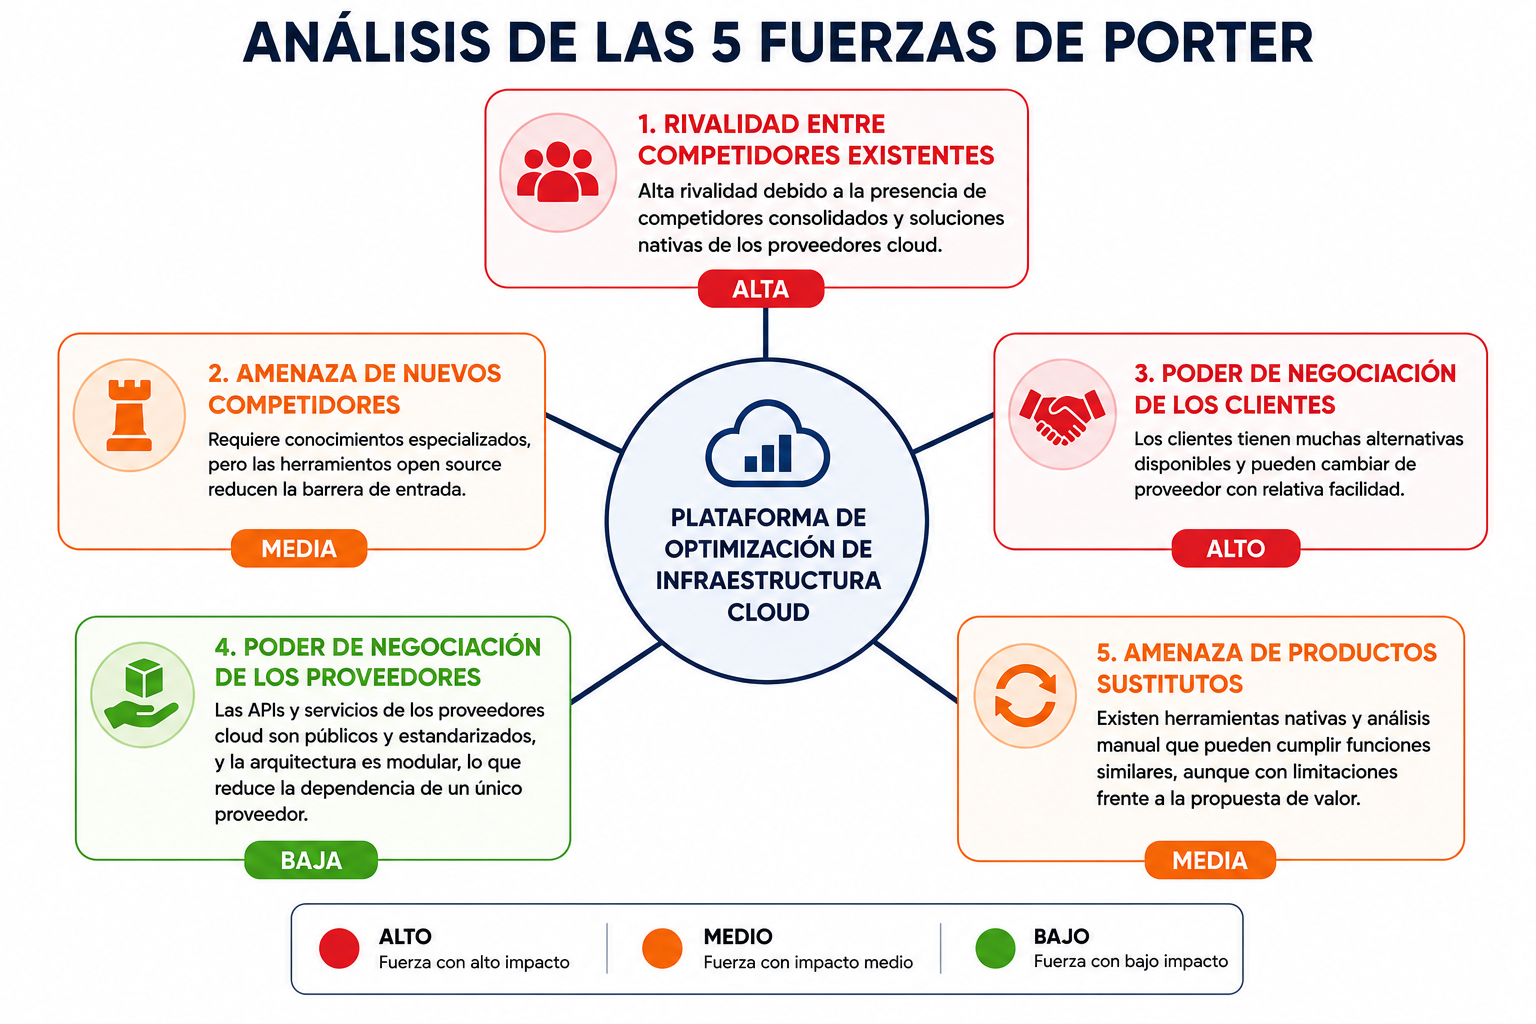
\includegraphics[width=0.9\textwidth]{media/image1.png}
\caption{Análisis de las Cinco Fuerzas de Porter}
\label{fig:porter}
\end{figure}

\subsection{Estrategia competitiva}

Del análisis realizado mediante las herramientas de marketing estratégico se desprende que el mercado de soluciones para la gestión de infraestructura cloud presenta un elevado nivel de competencia, impulsado principalmente por plataformas consolidadas como Datadog, Dynatrace, New Relic y las herramientas nativas de los principales proveedores cloud. No obstante, dicho análisis también permitió identificar oportunidades para el desarrollo de soluciones especializadas que atiendan necesidades específicas de optimización de infraestructura, diferenciándose de las plataformas orientadas principalmente a la observabilidad y el monitoreo continuo.

En este contexto, la estrategia competitiva de la solución se basa en la \textbf{diferenciación}. En lugar de competir directamente con herramientas de observabilidad de propósito general, la plataforma se posiciona como una solución especializada en la detección de recursos potencialmente mal dimensionados y en la generación de recomendaciones de optimización sobre Infraestructura como Código (IaC). Esta propuesta de valor combina técnicas de aprendizaje automático para identificar comportamientos anómalos con la generación automática de configuraciones en Terraform, facilitando la incorporación de las recomendaciones dentro de los procesos de administración y automatización de infraestructura.

Desde el punto de vista tecnológico, uno de los principales factores diferenciadores consiste en la obtención de información directamente desde las APIs del proveedor cloud, evitando la necesidad de instalar agentes propios sobre la infraestructura del cliente. Esta característica reduce la complejidad de implementación, disminuye el impacto operativo y favorece la adopción de la solución en organizaciones que administran entornos con políticas estrictas de seguridad o que buscan minimizar la incorporación de componentes adicionales en sus arquitecturas.

La estrategia comercial acompaña este posicionamiento mediante un modelo de distribución SaaS y un esquema Freemium, permitiendo que potenciales clientes evalúen el funcionamiento de la plataforma sin realizar una inversión inicial. Este enfoque reduce las barreras de adopción y facilita la incorporación progresiva de organizaciones de distintos tamaños, mientras que los planes de suscripción escalonados permiten que el crecimiento de los ingresos acompañe la expansión de la infraestructura administrada por cada cliente.

La estrategia propuesta no busca competir por amplitud de funcionalidades frente a las grandes plataformas de observabilidad, sino por la especialización en un problema concreto: la optimización inteligente del dimensionamiento de recursos cloud. La combinación de aprendizaje automático, generación de recomendaciones sobre Infraestructura como Código, ausencia de agentes propios y un modelo comercial de baja barrera de entrada constituye una propuesta de valor diferenciada que permite posicionar a la solución como una alternativa innovadora dentro del mercado de herramientas para la administración y optimización de infraestructuras cloud.

\section{Diagramas}

\subsection{Diagrama de componentes}

En este diagrama se visualiza la arquitectura de componentes de la plataforma, mostrando la interacción entre la interfaz web, los módulos encargados del procesamiento de las métricas y los componentes responsables de la detección y análisis de anomalías. Se representa el recorrido de la información desde la infraestructura de Huawei Cloud y el usuario, pasando por la API de backend, la recolección y transformación de los datos, el modelo de Isolation Forest y el motor de recomendaciones, hasta el almacenamiento de los resultados en PostgreSQL y su posterior utilización para la generación de reportes y visualización.

\begin{figure}[htbp]
\centering
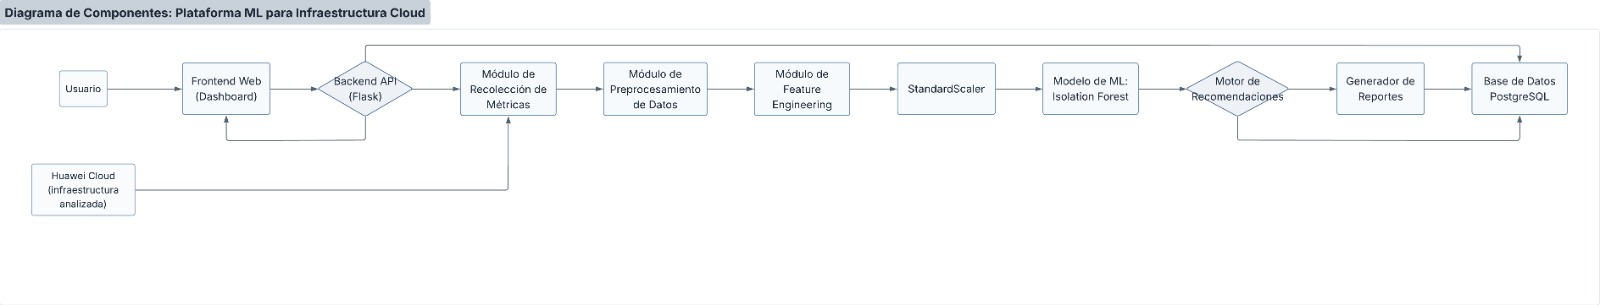
\includegraphics[width=0.9\textwidth]{media/image3.png}
\caption{Diagrama de componentes de la plataforma}
\label{fig:componentes}
\end{figure}

\subsection{Diagrama de flujo}

El siguiente diagrama presenta el flujo general de información de la plataforma, desde la obtención de las métricas de la infraestructura cloud hasta la generación y visualización de los resultados. Se detallan las principales etapas de procesamiento, incluyendo el preprocesamiento, la generación de características, la normalización y la detección de anomalías mediante Isolation Forest, seguida por el motor de recomendaciones cuando se identifica una instancia anómala. De esta manera, el diagrama permite visualizar de forma integral el recorrido de los datos dentro de la solución.

\begin{figure}[H]
\centering
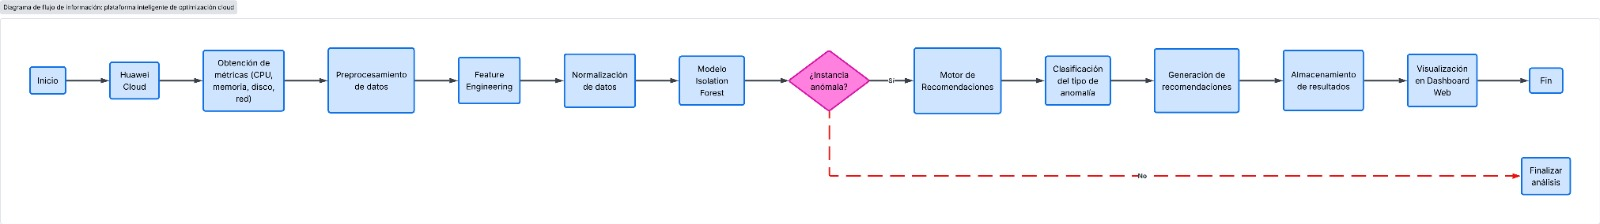
\includegraphics[width=0.9\textwidth]{media/image5.png}
\caption{Diagrama de flujo de la plataforma}
\label{fig:flujo}
\end{figure}

\subsection{Diagrama de arquitectura}

El diagrama de arquitectura presenta una visión general de la estructura tecnológica de la solución, mostrando la organización de los diferentes componentes y servicios que conforman la plataforma. Se observa la separación entre el frontend desarrollado con tecnologías web estándar, el backend implementado en Flask que actúa como intermediario entre la interfaz y los módulos de procesamiento, y los componentes especializados encargados de la comunicación con Huawei Cloud, la detección de anomalías mediante Isolation Forest y la generación de recomendaciones de optimización. Esta arquitectura modular permite que cada componente cumpla una función específica, facilitando la mantenibilidad del sistema y la incorporación de nuevas funcionalidades o proveedores cloud con un impacto mínimo sobre el resto de la solución.

\begin{figure}[H]
\centering
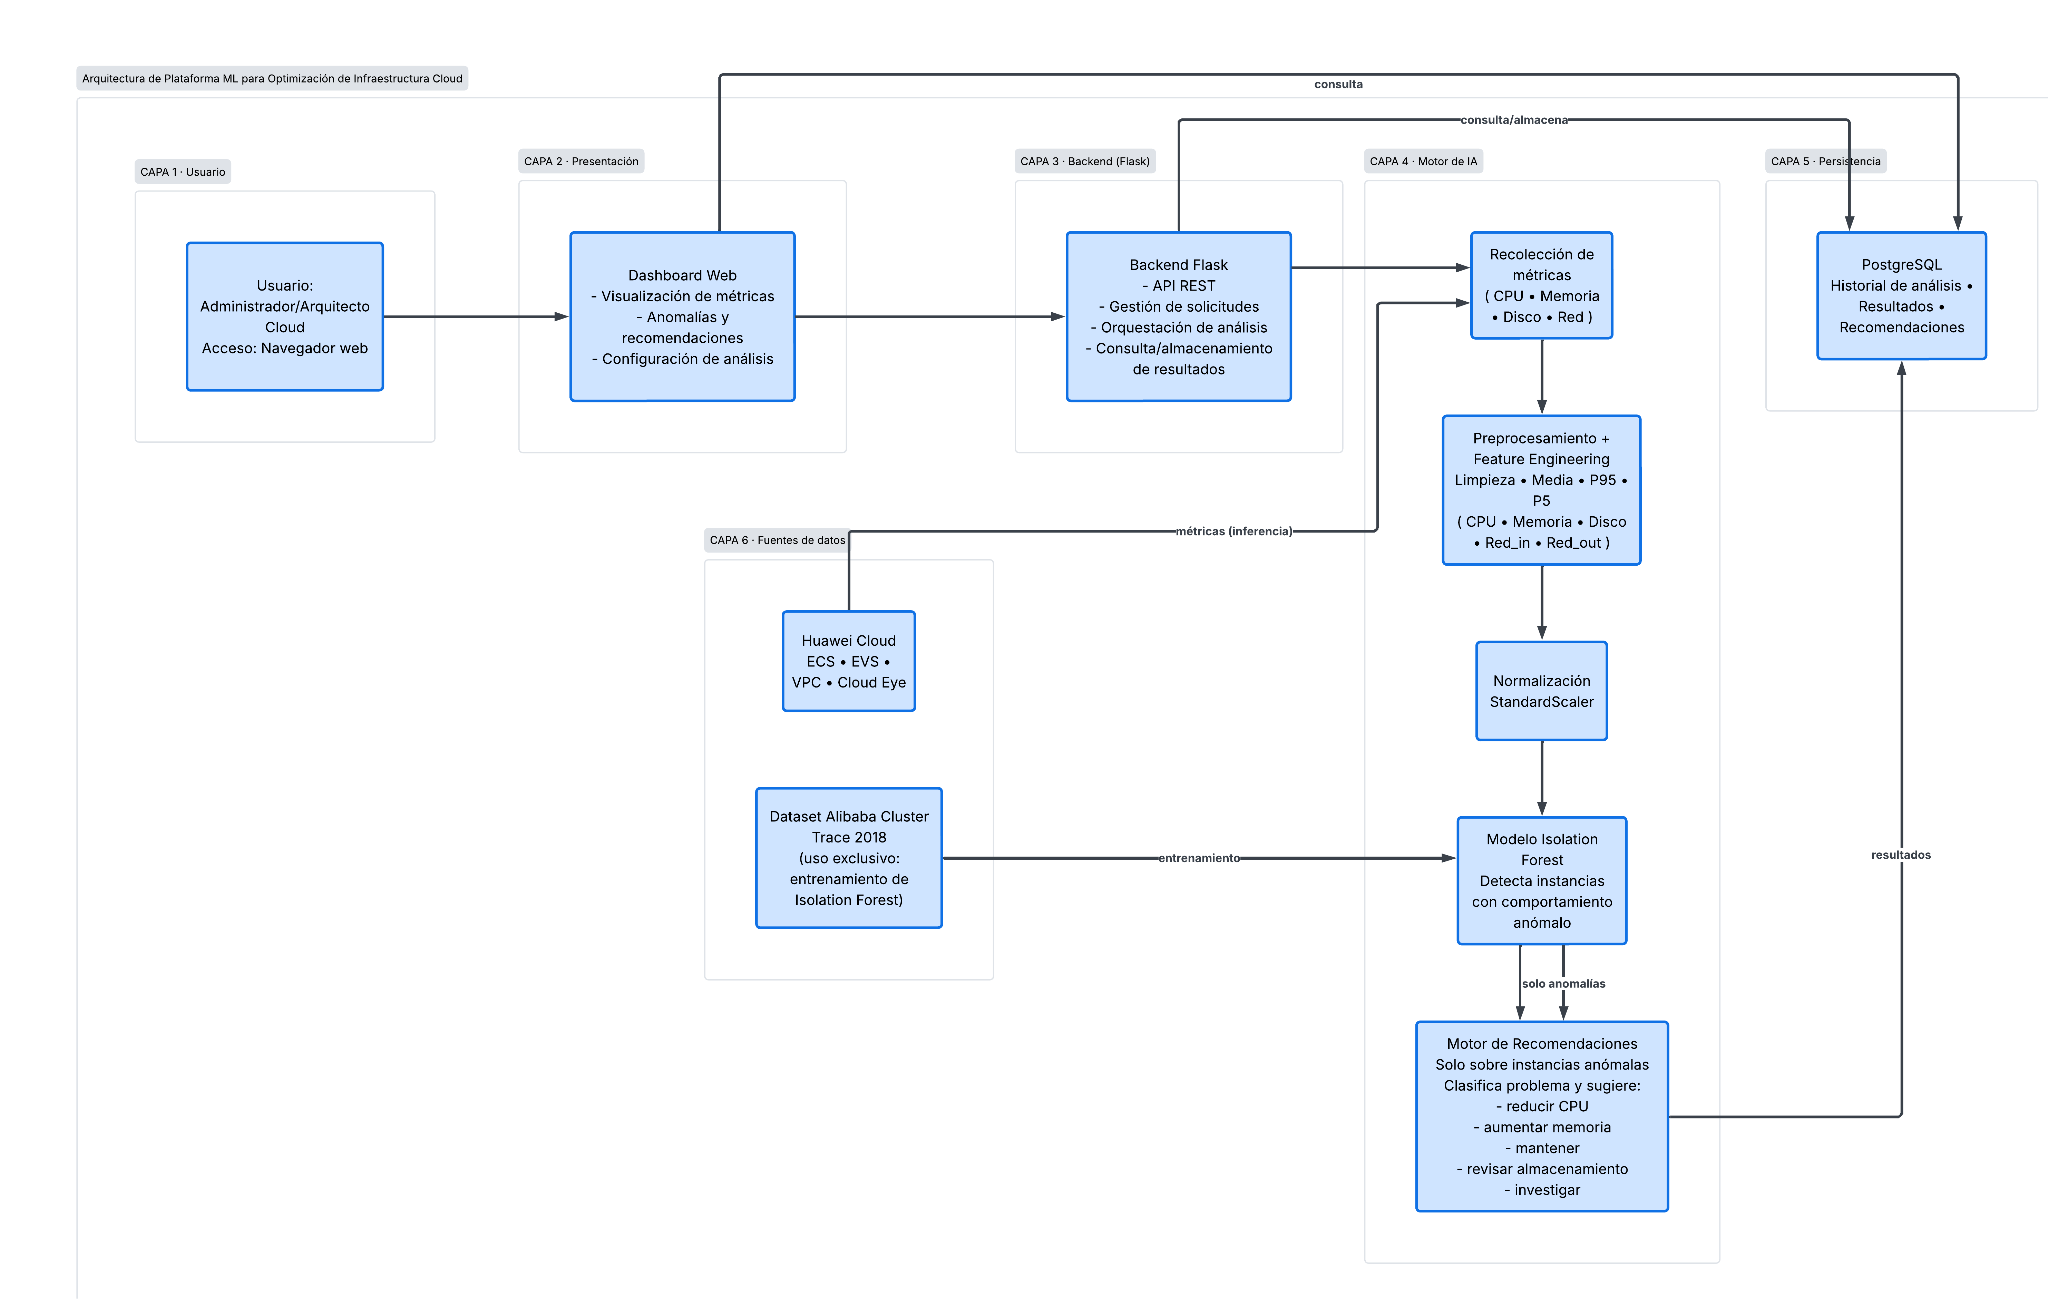
\includegraphics[width=0.9\textwidth]{media/image4.png}
\caption{Diagrama de arquitectura de la solución}
\label{fig:arquitectura}
\end{figure}

\subsection{Modelo Entidad-Relación}

El Diagrama Entidad-Relación presentado en la Figura representa el modelo de datos diseñado para la plataforma de optimización de infraestructuras cloud. El modelo establece una separación entre las distintas etapas de procesamiento de la plataforma. Las métricas representan el comportamiento observado de las instancias, los análisis representan las ejecuciones del modelo de detección, los resultados de anomalía representan las decisiones obtenidas mediante Isolation Forest y las recomendaciones representan las acciones de optimización derivadas de dichas detecciones. Esta estructura permite mantener la trazabilidad del proceso completo, desde los datos de utilización de los recursos hasta la generación de una recomendación de optimización.

\begin{figure}[H]
\centering
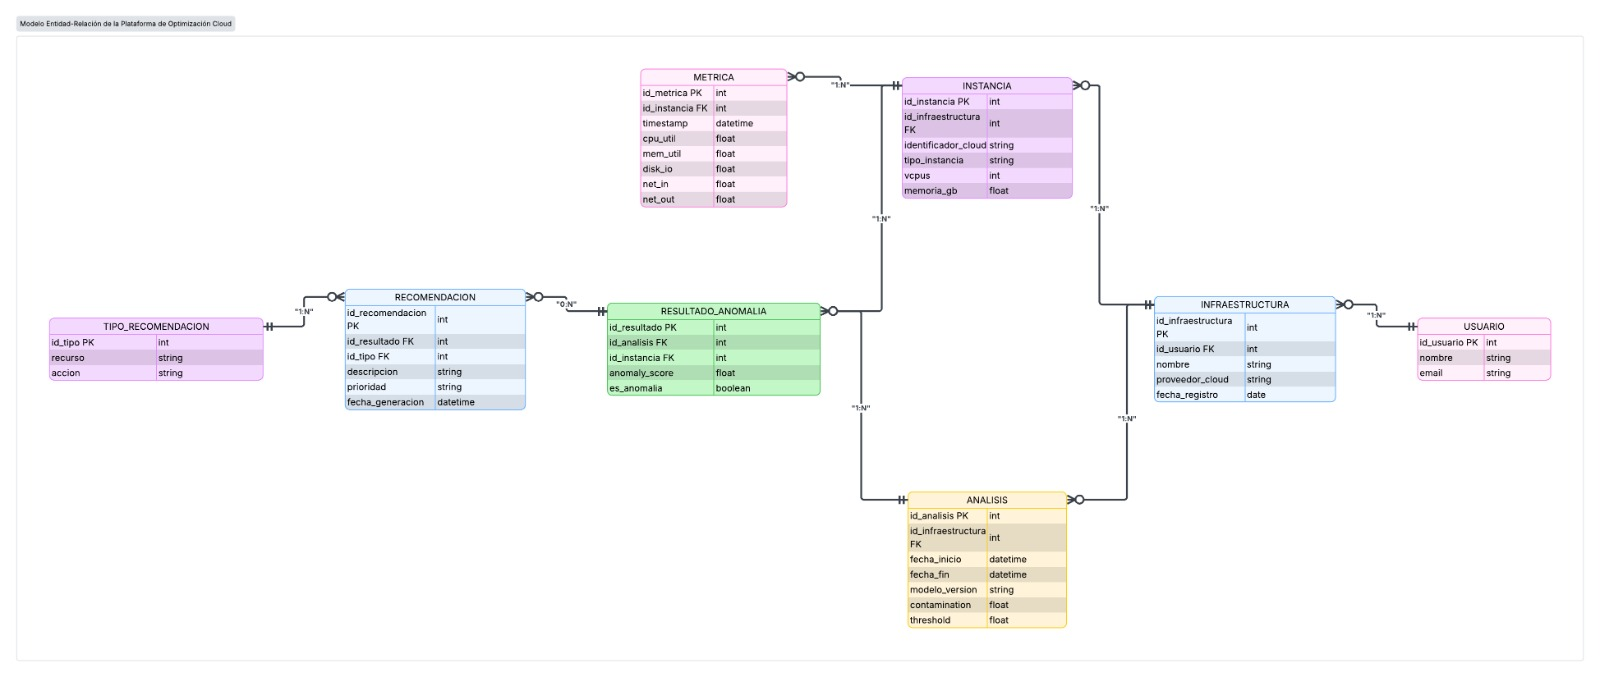
\includegraphics[width=0.9\textwidth]{media/image2.png}
\caption{Modelo Entidad-Relación de la plataforma}
\label{fig:er}
\end{figure}

\section{Tecnologías}

\subsection{Lenguaje de programación: Python}

Python constituye el lenguaje de programación principal de la solución
propuesta debido a su amplio ecosistema para el desarrollo de
aplicaciones web, procesamiento de datos y aprendizaje automático. En el
proyecto se emplea para implementar la lógica de negocio, el
procesamiento de métricas provenientes de la infraestructura cloud, el
entrenamiento y ejecución del modelo de detección de anomalías basado en
Isolation Forest, así como el desarrollo de los módulos encargados del
análisis de datos, la automatización de procesos y la validación
mediante pruebas unitarias. La elección de este lenguaje responde a su
versatilidad y a la disponibilidad de bibliotecas especializadas que
simplifican la implementación de soluciones de inteligencia artificial.

\subsection{Framework de desarrollo web: Flask}

El backend de la aplicación fue desarrollado utilizando Flask, un
framework web ligero para Python que permite construir aplicaciones
modulares con una baja sobrecarga de configuración. En esta solución,
Flask se utiliza para implementar la API REST que actúa como
intermediaria entre la interfaz web y los módulos de procesamiento,
facilitando la recepción de solicitudes, la ejecución del análisis de
las infraestructuras cloud y la devolución de los resultados al usuario.
Asimismo, el framework administra las rutas de la aplicación y la
renderización de las vistas utilizadas por el dashboard. La extensión
Flask-CORS complementa esta funcionalidad al habilitar el intercambio
seguro de información entre el frontend y el backend mediante la
configuración de políticas Cross-Origin Resource Sharing (CORS).

\subsection{Bibliotecas para aprendizaje automático y análisis de datos}

El desarrollo del sistema se apoya en un conjunto de bibliotecas
especializadas para el procesamiento de datos y la implementación del
modelo de inteligencia artificial. La biblioteca Scikit-learn constituye
el núcleo del sistema de detección de anomalías, ya que proporciona la
implementación del algoritmo Isolation Forest utilizado para identificar
patrones de utilización inusuales en los recursos de infraestructura.
Adicionalmente, esta biblioteca incorpora herramientas para la
normalización de características mediante StandardScaler y para la
evaluación del desempeño del modelo durante la etapa experimental.

Por otra parte, NumPy proporciona las estructuras de datos y operaciones
matemáticas necesarias para el procesamiento eficiente de grandes
volúmenes de información, permitiendo realizar cálculos vectorizados,
estadísticas descriptivas y percentiles sobre las métricas obtenidas de
las instancias cloud. Complementariamente, Pandas se utiliza para la
carga, limpieza, transformación y agregación de los datos provenientes
del conjunto Alibaba Cluster Trace 2018, además de facilitar la
generación de las características que posteriormente son utilizadas por
el modelo de aprendizaje automático. Finalmente, Matplotlib permite
representar gráficamente la distribución de las métricas, el
comportamiento de las anomalías detectadas y los resultados obtenidos
durante la evaluación experimental del sistema. Para reducir los tiempos
de ejecución, la persistencia del modelo entrenado y de los objetos de
preprocesamiento se realiza mediante Joblib, evitando la necesidad de
reentrenar el algoritmo en cada ejecución.

\subsection{Configuración del sistema}

La configuración dinámica del sistema se implementa mediante archivos en
formato YAML procesados a través de la biblioteca PyYAML. Esta solución
permite desacoplar los parámetros de configuración del código fuente,
facilitando la modificación de reglas de recomendación, umbrales de
detección y definiciones de los distintos tipos de instancias sin
necesidad de recompilar o alterar la lógica del sistema. Esta separación
favorece la mantenibilidad y la extensibilidad de la plataforma.

\subsection{Validación y aseguramiento de la calidad}

Con el objetivo de garantizar el correcto funcionamiento de los
diferentes módulos desarrollados, se emplea el framework Pytest para la
construcción de pruebas unitarias y de integración. Estas pruebas
permiten verificar el comportamiento del motor de recomendaciones, la
clasificación de anomalías y la correcta implementación de las reglas de
negocio. Adicionalmente, la extensión Pytest-cov se utiliza para medir
la cobertura del código fuente, identificando componentes que requieren
una mayor validación durante el proceso de desarrollo.

\subsection{Integración con Huawei Cloud}

La comunicación con la infraestructura cloud se realiza mediante los SDK
oficiales de Huawei Cloud, los cuales proporcionan acceso programático a
los distintos servicios utilizados por la plataforma. A través de estas
bibliotecas es posible consultar la información de las instancias
Elastic Cloud Server (ECS), recuperar métricas de monitoreo mediante
Cloud Eye, obtener información sobre los volúmenes administrados por
Elastic Volume Service (EVS) y acceder a la configuración de la red
virtual (VPC). Esta integración constituye la fuente principal de
información utilizada durante la etapa de inferencia del modelo,
permitiendo obtener las métricas necesarias para detectar anomalías y
generar recomendaciones de optimización sobre infraestructuras reales.

\subsection{Tecnologías del frontend}

La interfaz de usuario se desarrolla utilizando tecnologías web estándar
conformadas por HTML5, CSS3 y JavaScript. HTML5 proporciona la
estructura del dashboard y de las diferentes vistas utilizadas por la
aplicación, mientras que CSS3 se emplea para definir el diseño visual,
la adaptación a distintos tamaños de pantalla y la representación
gráfica del estado de las instancias analizadas. Por su parte,
JavaScript implementa la lógica del cliente, permitiendo consumir las
APIs REST desarrolladas en Flask, actualizar dinámicamente la
información mostrada al usuario e incorporar mecanismos de interacción
que facilitan la exploración de los resultados obtenidos durante el
análisis de la infraestructura.

\subsection{Algoritmo de detección de anomalías}

El componente central del sistema corresponde al algoritmo Isolation
Forest, una técnica de aprendizaje automático no supervisado diseñada
para detectar observaciones anómalas mediante la construcción de árboles
binarios generados aleatoriamente.

El componente de detección de anomalías tiene como objetivo identificar
instancias cuya utilización de recursos presenta un comportamiento
significativamente diferente respecto del patrón de utilización
aprendido a partir de un conjunto de datos de referencia. La finalidad
de esta etapa no consiste directamente en determinar qué recurso debe
ser redimensionado, sino en reducir el universo de instancias que
posteriormente serán evaluadas por el motor de recomendaciones. De esta
manera, el modelo de aprendizaje automático funciona como una primera
etapa de filtrado, mientras que la determinación de una posible acción
de optimización queda a cargo del módulo de recomendaciones.

El modelo utiliza como fuente de entrenamiento el conjunto de datos
Alibaba Cluster Trace 2018, que contiene información de utilización de
recursos obtenida a partir de una infraestructura de producción. A
partir de las métricas disponibles se construye una representación de
cada instancia que posteriormente será utilizada como entrada del
algoritmo.

Las variables consideradas corresponden a la utilización de CPU,
memoria, disco, tráfico de red entrante y tráfico de red saliente.
Debido a que las métricas originales representan observaciones
individuales obtenidas a lo largo del tiempo, se realiza una etapa de
transformación que permite representar el comportamiento de cada
instancia mediante características estadísticas.

Para cada una de las métricas se calculan tres características: media,
percentil 5 y percentil 95. La media permite representar el nivel
habitual de utilización del recurso, mientras que los percentiles
permiten incorporar información sobre los niveles bajo y alto de
utilización sin depender exclusivamente de valores extremos. De esta
forma, cada instancia queda representada mediante un conjunto de
características que describe tanto su utilización habitual como los
niveles de utilización que alcanza en situaciones de menor y mayor
demanda.

Con cinco métricas y tres características derivadas para cada una, la
representación final utilizada por el modelo está compuesta por 15
variables. Esta transformación permite que Isolation Forest trabaje con
una representación homogénea de las instancias y no directamente con las
series temporales originales.

Una vez construidas y normalizadas las características, se procede al
entrenamiento del modelo Isolation Forest. El algoritmo construye un
conjunto de árboles de aislamiento mediante particiones aleatorias del
espacio de características.

El modelo utilizado se configura con 100 árboles, buscando obtener una
representación estable del espacio de características a partir de
múltiples particiones aleatorias. Asimismo, se establece una semilla
aleatoria fija para garantizar que los experimentos puedan ser
reproducidos bajo las mismas condiciones.

Durante el entrenamiento se establece el parámetro contamination,
utilizado por Isolation Forest para determinar la proporción esperada de
observaciones anómalas dentro del conjunto de entrenamiento.

Una vez finalizada la etapa de entrenamiento, el modelo Isolation Forest
queda disponible para analizar nuevas infraestructuras sin necesidad de
volver a entrenarse para cada análisis. Durante la etapa de inferencia,
el sistema obtiene las métricas de utilización correspondientes a las
instancias de la infraestructura que se desea evaluar. Estas métricas
constituyen los datos de entrada sobre los cuales se aplicará el modelo
previamente entrenado.

El proceso de inferencia comienza aplicando a los datos obtenidos el
mismo procedimiento de transformación utilizado durante el
entrenamiento. Para cada instancia se calculan las características
correspondientes a las métricas de CPU, memoria, disco, tráfico de red
entrante y tráfico de red saliente. A partir de cada métrica se obtienen
la media, el percentil 5 y el percentil 95, generando nuevamente las 15
características que representan el comportamiento de la instancia.

Una vez completado el preprocesamiento, las características normalizadas
son introducidas en el modelo Isolation Forest. El algoritmo recorre los
árboles construidos durante la etapa de entrenamiento y determina qué
tan fácilmente puede aislar cada observación respecto del conjunto de
referencia.

Isolation Forest asigna a cada instancia un anomaly score, que
representa el grado en que su comportamiento se diferencia del patrón
aprendido durante el entrenamiento. Este valor permite establecer una
medida continua de anomalía antes de realizar la clasificación final.

En la implementación devuelve el puntaje de cada observación. Los
valores más bajos representan observaciones con un comportamiento más
susceptible de ser considerado anómalo, mientras que valores
relativamente mayores corresponden a observaciones más próximas al
comportamiento considerado normal.

A partir de los puntajes obtenidos, cada instancia es clasificada como
normal o anómala. Para realizar esta clasificación se utiliza el umbral
asociado al modelo, determinado durante su configuración y entrenamiento
en función del parámetro contamination.

Una instancia cuyo puntaje se encuentra por debajo del umbral
establecido es clasificada como anomalía, mientras que aquellas cuyo
puntaje se encuentra por encima del límite son consideradas normales.
Esta separación permite transformar el resultado continuo producido por
Isolation Forest en una decisión binaria que puede ser utilizada por las
etapas posteriores del sistema.

\subsection{Arquitectura del software}

La aplicación adopta una arquitectura modular que organiza sus
componentes según su responsabilidad funcional. Los módulos de
adquisición y preprocesamiento de datos son responsables de obtener y
preparar las métricas para su análisis, mientras que el módulo de
aprendizaje automático implementa la detección de anomalías mediante
Isolation Forest. De forma complementaria, el motor de recomendaciones
procesa exclusivamente las instancias identificadas como anómalas y
genera propuestas de optimización de recursos. Finalmente, el sistema
incorpora módulos de integración con Huawei Cloud, generación de
reportes y una aplicación web desarrollada en Flask para la interacción
con el usuario. Esta organización modular favorece la mantenibilidad,
escalabilidad y reutilización de los distintos componentes del sistema.
